%\documentclass[letterpaper]{article}
\documentclass{chi2009}

%\usepackage{aaai}
%\usepackage{times}
%\usepackage{helvet}
%\usepackage{courier}
\usepackage{todonotes}
\usepackage{graphicx}
\usepackage{tabularx}
\usepackage{caption}
\usepackage{subcaption}
\usepackage{hyperref}
\usepackage{cite}

\usepackage[T1]{fontenc}
\usepackage{textcomp}
\usepackage{times}
%\usepackage[minionint,mathlf]{MinionPro}
\renewcommand{\sfdefault}{Myriad-LF}

%\usepackage[usenames]{color}
\usepackage[protrusion=true,expansion]{microtype}
\usepackage{layout}
\usepackage{xspace}
\usepackage{multirow}
\usepackage{array}
\usepackage{colortbl}
\usepackage{enumitem}
\usepackage{url}
\usepackage{booktabs}
%\usepackage{sfmath}
\frenchspacing

\pdfinfo{
/Title (How Do Professional and Amateur Reviewers Differ?)
/Subject (anonymous)
/Author (anonymous)}
\setcounter{secnumdepth}{0}  
\begin{document}
% The file aaai.sty is the style file for AAAI Press 
% proceedings, working notes, and technical reports.
%

\skip\footins=1.5\bigskipamount     % Determine the space above the rule
\renewcommand*{\footnoterule}{
  \kern-3pt
  \hrule width 2in
  \kern 2.6pt
  \vspace{\smallskipamount}       % The additional space below the rule
}
\renewcommand\arraystretch{1.3}

\makeatletter
\def\url@leostyle{%
  \@ifundefined{selectfont}{\def\UrlFont{\sf}}{\def\UrlFont{\small\ttfamily}}}
\makeatother
%% Now actually use the newly defined style.
\urlstyle{leo}

% don't hyphenate so much - default = 200, max (never hyphenate) = 10,000
\hyphenpenalty=100
\tolerance =200

% pagebreak penalties
\widowpenalty=10000 % penalty for a lone line at the top of the page
\clubpenalty=10000 % penalty for a lone line at the bottom
\brokenpenalty=10000 % penalty for breaking a word across pages

\markright{\today}

\title{Crowds and Critics: How Professional and \\ [0.5ex]Amateur Reviews
Differ on Metacritic}
\author{
%anonymous\\
%location\\
%address 1\\
%address 2\\
}
\maketitle

\begin{abstract}
Both professional and amateur reviews can substantially shape
how products fare in the marketplace. Yet, we know little about how these two
viewpoints compare. 
In this paper, we bridge this gap by contrasting professional and
amateur reviews within the 
domain of videogames. Examining nearly 200K 
reviews from the popular site Metacritic, we find
professionals favor phrases describing the broader market, while
amateurs emphasize social aspects of playing games. Amateurs skew
towards higher scores, but are the primary source of low
scores; that is, they show considerably more variance. 
However, both groups express the same average levels of sentiment.
Finally, regressing future videogame sales on reviews, we
find that a combination of professional scores, volume of professional
reviews, and volume of amateur reviews provides a moderately powerful
predictive model for future game sales. This is the first work
we know of to systematically contrast professional and amateur
reviewers, addressing a question at the heart
of many contemporary debates: How do crowds and domain
specialists compare?

\end{abstract}


\section{Introduction}
\vspace{6pt}
\begin{quote}
\small
Do not buy this game. Do not rent this game, do not look at this game on the shelf, don't even think about this game lest someone at Ubisoft find out and they prep a Just Dance 2. Such would be the end of all things, mark my words.

--- \textit{Just Dance} professional review; score: 20/100 % IGN is reviewer :)
\end{quote}

\begin{quote}
\small
Screw professional reviews. My wife and I have played DDR, Dancing with
the Stars, We Cheer, that other Wii game with the microphone---all terrible. This game is great because it is fun. End of story. All you pro reviewers are wrong.

--- \textit{Just Dance} amateur review; score: 10/10
\end{quote}

The Wii game \textit{Just Dance} released to near-universal
critical derision. With a ``metascore'' of 49/100 based on 21
professional reviews, the review site Metacritic gives the game its worst
possible rating category. Yet amateur reviewers loved it---yielding an average 8/10 score over 107 ratings. And at the
time of this writing, \textit{Just Dance} has gone on to sell 6.9M units
and spawn a franchise with three sequels and versions on all major
videogame platforms. While the case of \textit{Just Dance} is in many
ways exceptional, it does suggest a question: Just how divergent are professional product reviews from amateur ones?

Particularly in the entertainment industry, the opinions of elite
critics and journalists hold sway. Professional film critics
such as The New York Times's A. O. Scott are regarded as important
for recognizing hidden gems and over-hyped flops. Yet despite this
widespread regard, relatively little science exists on how indicative
these professionals' opinions are for market success. Nor do we know 
how they differ from the opinions of ordinary consumers.

In this paper, we bridge this gap by comparing professional critics and
amateur reviewers within the context of videogame reviews. Who knows the
market best, professionals or amateurs? Who will best predict a
product's eventual success or failure? Do professionals and amateurs
differ in their expressions of sentiment? How do professionals and
amateurs describe products when reviewing? While previous work has
investigated the question of predicting sales from reviews
\cite{chevalier2003effect,dellarocas2007exploring,duan2008online,forman2008examining,gruhl2005predictive,liu2001word,yu2012mining},
the differences between professionals and amateurs have received little
attention. With this work, we believe we address a question at the heart
of many contemporary debates: How do crowds compare to domain
specialists and who is more effective for predicting future outcomes?

We bring together a corpus of 197K reviews from 
the review aggregator Metacritic with sales data on 7K videogames. In summary, we find that a
combination of professional score, volume of professional reviews,
and volume of amateur reviews effectively predicts game sales. Amateurs
skew toward higher review scores than professionals, but also
provide the main source of low review scores. That is, they show more
variation. Amateurs and professionals also show very similar levels of
average review subjectivity and polarity; however, amateurs tend toward
more extreme and more varied expressions of sentiment. Finally,
professionals and amateurs systematically differ in their language, with
experts focusing on market factors and amateurs focusing on
social aspects of playing games.

First, we present an overview of our corpora, characterizing the
distribution of professional and amateur review scores and sentiment
expressions. Next, we model total sales-to-date as a function of 
professional and amateur review scores before a game's release. Finally,
we train classifiers on review text to find key words differentiating
professional and amateur reviews. We conclude this paper by discussing
implications this work has for CMC theory and for practical
issues, such as combining reviews from professionals and amateurs.

\section{Related Work}
Technologies like wikis, blogs, discussion forums, and online review
venues have enabled new distributed forms of knowledge production,
information sharing, social support, and opinion aggregation \cite{Benkler2006Wealth}. People read movie critics' reviews of new films; now Netflix and Amazon recommend movies based on what fellow moviegoers like. Subject matter experts wrote encyclopedias; now there is Wikipedia. People with health conditions went to doctors; now there's PatientsLikeMe. 

In addition to these commercial examples, amateurs have proven valuable
across many domains, providing insight and creative energy to fields as diverse as astronomy, mathematics and animation \cite{cooper2010predicting,cranshaw2011polymath,kanefsky2001can,luther2013redistributing}.
However, professionals have traditionally provided many of these services, prompting the question: what value are professionals in these systems?
%Wikipedia offers a case in point. There is significant ongoing controversy about the role of subject matter experts: are external credentials relevant? Should a PhD give you special editing privileges? Historically the answer has been ``no'', although there are recent moves away from this position (Wikipedia Public Policy Initiative 2010). 
%Larry Sanger, a Wikipedia co-founder, has been critical of this position, arguing in favor of finding a role for accredited experts (Sanger 2009). He started his own online encyclopedia to pursue this approach (Citizendium.org).  
%More recently, the Association for Psychological Science has begun an effort to encourage and guide academic psychologists to edit Wikipedia articles about psychological topics (APS Initiative). 
Efforts have varied in how they integrate professionals with amateurs.
Several prominent Citizen Science projects feature distinct roles for professionals (scientists) and amateurs (citizens/laypeople). For example, birders participating in the eBird project enter their observations of birds. Then, ``automated data quality filters developed by regional bird experts review all submissions'' and ``local experts review unusual records that are flagged by the filters'' \cite{sullivan2009ebird}.
On the Encyclopedia of Life anyone can contribute but materials from
unvetted contributors are initially marked as unreviewed. EOL curators
are ``professional scientists'' and ``experienced citizen scientists'' who have applied and been approved \cite{encyclopediaoflife}. 
Metacritic aggregates review scores from a selected set of professional reviewers for movies, games, television, and music. These review scores are compiled into an aggregate ``metascore'' that measures the overall quality of a product. Amateurs may also post reviews to the site that are displayed alongside these professional reviews, but are not counted toward the overall metascore of a title.

Quantifying the value of amateur activities is a challenging task. 
%The increasing prevalence and ease of access to social media data has led to a rise in research predicting real-world economic, political, and other events \cite{asur2010predicting}. 
Predicting books sales \cite{gruhl2005predictive,chevalier2003effect}, film box office sales \cite{dellarocas2007exploring,yu2012mining}, and (to a lesser extent) videogame sales \cite{ehrenfeld2011predicting,marcoux2009hybrid} from online reviews or blog chatter have all attracted attention as ways of grounding the value of amateur reviewers. In early work in this area, Gruhl et al. demonstrated blog chatter can predict spikes in book sales rank on Amazon \cite{gruhl2005predictive}. Chevalier and Mayzlin found improvements in review scores on book sales sites precede increases in book sales \cite{chevalier2003effect}. Forman, Ghose, and Wiesenfeld found that increases in product reviews including identity-descriptive information associated with subsequent increases in online book sales \cite{ghose2007designing}.

Predicting box office sales has found volume of mentions on blogs or Yahoo!'s movie pre-release discussion forums can predict film box office sales \cite{liu2001word,duan2008online}. Results conflict, however, on whether review score averages are \cite{dellarocas2007exploring,hennig-thurau2012movie-reanalysis} or are not \cite{liu2001word,duan2008online} predictive of sales, beyond the power of pure volume of reviews.
%Hennig-Thurau et al. distinguish online review influence from predictive powers, finding reviews have a weak impact on short-term sales and a non-linear effect of higher scores disproportionately increasing long-term sales \cite{hennig-thurau2012movie-reanalysis}. We observe a similar non-linear relationship in domain of videogames.
Sentiment has also often proven useful in predicting sales. 
Yu et al. found sentiment expressed in blog posts can improve an autoregressive model through a carefully chosen lexicon of sentiment-laden words \cite{yu2012mining}. 
Specialized classifiers that differentiate product description text from opinion related text were shown to improve sales prediction by Ghose and Ipeirotis \cite{ghose2007designing}. 
We address the question of review subjectivity and its relation to sales prediction and reviewer expertise, finding no strong predictive powers in the domain of videogame sales.

Few of these early works explicitly examine whether and how different types of reviewers produce varying review scores. 
Dellarocas et al. note a weak correlation between amateur and professional film reviews and find that removing professional review information (average score only) is slightly less detrimental to their model's performance than removing amateur review information (a combination of average score, number of reviews, entropy of review gender distribution, entropy of reviewer age distribution) \cite{dellarocas2007exploring}. 
Kim et al. find frequency of online word-of-mouth mentions and expert review valence are predictive of box office sales \cite{kim2013moviewom}.
Plucker et al. compare student, online novice, and professional film reviewers, finding greater experience watching films correlates with increased similarity to professional reviews \cite{plucker2009pro-novice-eval}. 
Earlier studies of online reviewing examined amateur reviewers in terms of their motivations for reviewing \cite{gilbert2010deja,diakopoulos2011news-discourse,xu2012critique} and characteristic language used in videogame reviews in particular \cite{zagal2011natural}. We complement this work through an assessment of the differences between professional and amateur reviewers through examining review volume, score, and sentiment rating in a linear model that allows direct comparison of predictive power. Further, our analysis of review text and score distributions provides in-depth insight into how professional and amateur reviews differ. Rather than characterize amateur reviewer traits in isolation we seek to understand how they compare against professionals.

Our work broadens previous analyses of videogame sales that have been limited to smaller subsets of games or sources for review data. Ehrenfeld's thesis found volume of game mentions on the NeoGAF online game discussion forum is predictive of game weekly sales in a support vector regression model \cite{ehrenfeld2011predicting}. Marcoux and Selouani employed an autoregressive neural network model to predict games sales from review scores, volume, and related features using data from the IGN videogame news and reviews website after first performing nonlinear transformations of the model data \cite{marcoux2009hybrid}.
Compared to these approaches we examine a much larger set of
games\footnote{Ehrenfeld does not report the number of games used in his
analysis, but limits to data over the course of 42 weeks of releases,
which is a subset of our total corpus spanning 425 weeks. Marcoux and
Selouani examine 74 games, while we examine 860 or 600, depending on the
model.},
compare professional and amateur reviews, and draw from a longer-term and larger set of reviews that aggregate over websites. Our results are directly interpretable in terms of relative feature impact in linear models.


\section{Method}

%We used the python Scrapy package\footnote{http://scrapy.org/} to scrape all amateur and professional reviews for videogames from the Metacritic website\footnote{http://www.metacritic.com/} up through December 7 2012. 
We crawled every amateur and professional review for video-games on the
Metacritic website\footnote{http://www.metacritic.com} through December
7, 2012. We chose videogames both because it is a relatively
under-studied product domain (movies and books have received far more
research attention), and also because videogames fit into a broader
research project. 
For every game we collected the following information: console (the
hardware the game software was made for), title, publisher (company
responsible for distributing the game), developer (studio responsible
for making the game), release date, current metascore, current average
``user'' (amateur) score, genre (according to Metacritic), and ESRB
rating (an age-appropriateness rating). Note that some titles may appear on multiple consoles. We treat these as separate games as they reach potentially different audiences and may vary in their implementation. 

From every game we also collected all amateur and professional reviews,
including their text, review score, time of review, and a flag
indicating whether the review came from a amateur or professional.
Metacritic converts professional review scores from many formats (such
as letter grade, 0-10 range, 0-100 range) into a 0-100 score. Amateur
reviews are limited to a 0-10 score range. For comparison, we divide all professional scores by 10 to have all reviews on a 0-10 scale. Metacritic only provides summary excerpts from professional reviews and we limited ourselves to this text to make review length more comparable between amateurs and professionals. Our final corpus consists of 197,383 reviews: 138,843 from professionals and 58,540 from amateurs. Of these, 4,331 professional and 729 amateur reviews covering 958 games were in the first 10 weeks prior to the release of the game---these were used in our future sales prediction tasks.

\subsection{VGChartz sales data}
For sales data we scraped information from the VGChartz website\footnote{http://www.vgchartz.com}. VGChartz tracks weekly, annual, and lifetime game sales data from a variety of outlets and is primarily targeted toward sales of games in the United States. Their data is most accurate for console games (rather than computer or mobile phone), so we limit ourselves to examining the following consoles using only US sales data: Sony's PlayStation 3 (PS3), PlayStation Portable (PSP) and Vita; Nintendo's Wii, DS, and 3DS; and Microsoft's Xbox360. These consoles are considered to make up the current generation of videogame hardware and are the primary game console distribution platforms. VGChartz typically only records the first 10 weeks of game sales at weekly granularity, limiting our analysis to these weeks. We collected total lifetime sales-to-date for 7,467 games and weekly sales for the first ten weeks of game sales for 4,902 games.

\subsection{Statistical Methods}
We apply three different methods to compare and contrast professional
and amateur reviews: regressing sales on reviews, extracting sentiment
from text, and searching for keywords distinguishing professionals from
amateurs.

\subsubsection{Sales prediction regression}
Our sales predictions investigated: 
\begin{enumerate}
%\item predicting total lifetime sales-to-date using the full professional and amateur review database (total vs all)
\item predicting total lifetime sales using reviews in the 10 weeks prior to the release of a game (total vs pre-10)
\item predicting net first 10-week sales using the same pre-release review subset (10-week vs pre-10)
\item predicting lifetime sales comparing metascore, professional, and amateur review scores using all available reviews (total vs meta)
\end{enumerate}
%(1) predicting total lifetime sales-to-date using the full review database, (2) predicting total lifetime sales-to-date using only reviews in the 10 weeks prior to the release of a game, (3) predicting net first 10 week sales using the same pre-release review subset, and (4) predicting lifetime sales using the full review database augmented with metascore information (Table \ref{tab:regression_models} summarizes our models). 
Predictive accuracy was assessed through mean squared error (MSE)
computed with leave-one-out cross-validation via bootstrapped resampling with R's boot package\footnote{http://cran.r-project.org/web/packages/boot}.
%To predict lifetime sales data we constructed a robust linear regression model for logged lifetime game sales based on median review scores using R's MASS package\footnote{http://cran.r-project.org/web/packages/MASS/}.

\begin{table*}[tb]
\centering
\small
\sffamily
%\begin{tabularx}{\linewidth}{|c|c|c|c|c|c|c|c|}
\begin{tabular}{llllllll}
predicted variable & review set & total games & $R^2$ & MSE & null deviance & control deviance & model deviance \\ 
%\hline lifetime sales-to-date & all & 6809 & 0.405 & 0.600 & 6807 & 6130 & 4048\\ 
\midrule lifetime sales-to-date & pre-10 & 600 & 0.360 & 0.669 & 562 & 500 & 360\\ 
net first 10 week sales & pre-10 & 600 & 0.421 & 0.642 & 599 & 502 & 347\\ 
%\hline lifetime sales-to-date & divided & 2902 & 0.472 & 0.537 & 2897 & 2655 & 1528\\ 
lifetime sales-to-date & meta & 839 & 0.446 & 0.586 & 839 & 736 & 464\\ 
lifetime sales-to-date & meta sub & 839 & 0.430 & 0.599 & 839 & 736 & 478\\ 
%\end{tabularx}
\end{tabular}
\caption{Linear regression models. Review set indicates which subset of reviews were used:
%``all'' indicates using the full review database,
``pre-10'' indicates only reviews from the 10 weeks prior to the launch of the game,
%``divided'' indicates all games with reviews from both amateurs and professionals with separate predictors for amateur and professional review features,
``meta'' indicates the full review database and metascore information, and ``meta sub'' is the same model without metascore information. 
Mean squared error (MSE) values are from leave-one-out cross-validation of models. Null deviance reports null model deviance; control deviance includes only console, game genre, and maturity (ESRB) rating as predictors; model deviance uses full set of predictive variables including controls. All deviance differences were significant ($\chi^2$ test $p < 0.001$).}
\label{tab:regression_models}
\end{table*}

After matching game reviews to sales data using game titles and consoles, we had lifetime sales data for 6,809 games, and weekly sales for 600 games. Of the 6,809 games with lifetime sales 2,902 had both professional and amateur reviews, while 839 additionally had metascores. Metascores are only assigned when at least four professional critics approved by Metacritic have reviewed the game.

We took a conservative approach of only keeping exact game title matches
between Metacritic and VGChartz data without manipulating titles (e.g.,
using lowercase versions or removing punctuation). We believe it is better to have a slightly smaller dataset than misattribute review scores to different games. All games were matched by a concatenation of title and game console, as games on different consoles vary in implementation, release date, and audience demographics. 

Reviews and sales data were aligned based on weeks since release. Reviews were binned into weekly periods based on time since the release of the game. For example, all reviews within 7 days of the game's stated release date (for that console) were binned into the first week. Sales values were logged to get closer to normality. From reviews we constructed features for mean and median review scores, number of reviews, and review length.

\subsubsection{Review sentiment extraction}
We employed the Pattern toolkit\footnote{http://www.clips.ua.ac.be/pages/pattern} to analyze review text sentiment. For every review, we parse the text into sentences, compute per-word sentiment (both polarity and subjectivity) and compute the per-review mean, median, minimum, maximum, and variance of sentiment values. Subjectivity values measure the extent to which a text conveys an opinion. Polarity values estimate that opinion as positive or negative. Below we refer to these per-sentence aggregation values as the review ``mean'', ``median'', ``minimum'', ``maximum'', or ``variance'' of polarity or subjectivity. ``Overall'' subjectivity and polarity measure the review text as a whole, instead of computing per-sentence values and aggregating them. Considering these metrics allowed us to consider expressions of average review sentiment (median, overall), skew in review sentiment (mean vs median, variance), or extreme review sentiment (minimum, maximum). All features (including score features above) were centered and scaled by subtracting their mean and dividing by their standard deviation.

\subsubsection{Reviewer text analysis}
We examined the power of review text words to classify reviewers as professionals or amateurs (labeled 0 and 1, respectively) using penalized binomial regression with a lasso penalty to favor the use of a small set of terms.
We prepared our review texts using several standard methods from text analysis using the R programming language package tm.\footnote{http://cran.r-project.org/web/packages/tm} We removed whitespace, punctuation, numbers not part of words, and common English words. All text was lowercased and stemmed to group similar words. We tokenized the reviews into single words, requiring words be at least 3 letters long and appear in at least 10 documents. After constructing a full corpus with 86,376 terms we removed the most sparse terms to produce a set of 2,581 terms.

For binomial regression we used R's glmnet package\footnote{http://cran.r-project.org/web/packages/glmnet} for generalized linear models. These models account for collinearity of terms (their frequent appearance together altering relative importance) and can control for sparsity (relative infrequency of terms). Controlling collinearity is important to prevent overweighting words that often appear together. Accounting for sparsity enables the model to exclude terms with little predictive power, yielding a smaller and more interpretable set of results. We used a lasso penalty to encourage the model to use the smallest set of terms possible. The parsed text corpus was used to examine review text but not for sales prediction---future work should explore which text features are most predictive of game sales and how they relate to reviewer types.

% % note: I did this but the results weren't all that interesting. might be better with bigrams + trigrams


\section{Results}
Before describing results on our prediction tasks it is important to understand the characteristics of the review and sales corpora we collected. It is not apparent \textit{a priori} how Metacritic amateurs behave compared to the professionals whose reviews are featured on the site. Below we explore how professionals and amateurs differ in aggregate scoring and review sentiment expressions.

\subsection{Review scores}
Amateurs and professionals show clear differences in review score assignment (Figure \ref{fig:revscore_console}). Professionals tend to provide reviews distributed more tightly around a mean 7.2 and median 7.5 score, while amateurs show greater variation with a mean 7.4 and median 9.0 score (Table \ref{tab:review_pol_subj}). A Wilcoxon test found these differences to be significant (p $< 0.001$). Amateurs favor providing higher scores than professionals, but are the only ones likely to provide low review scores, seen by a larger portion of the cumulative review distribution on lower scores (Figure \ref{fig:game_score}). Amateurs tend to provide few reviews on any single game, while professionals tend to more frequently provide many reviews (Figure \ref{fig:game_reviewnum}). Thus, amateurs tend to focus on a few high-profile games, but provide a wider range of scores than professionals. 

Factors relating to professionals' role and amateurs' motivations may
explain these differences. Professionals are often under threat of
blacklisting for providing low review scores and have a reputation to
preserve by not consistently giving high review scores. Game
distributors are also unlikely to provide reviewers with free game
copies for review if they anticipate low ratings, while professionals
are unlikely to review low profile and low quality titles that will not
drive traffic to their websites. These factors could combine to skew professionals towards reviewing games generally favorably without providing overly positive reviews.

Amateurs, by contrast, are most likely to review games that provided a great or terrible experience \cite{gilbert2010deja}. As Metacritic is a major game review outlet, reviewers are likely to provide high scores to games they enjoyed, while attacking games they found poor quality or a waste of money. ``Fanboy'' culture also likely plays a role in driving reviewing behavior. Our text analysis results corroborate these findings, showing amateurs often describe product value, while professionals focus on potential purchaser game feature interests and demographics (see below). Both amateur and professional reviewers acknowledge the strongly split gaming demographics, shown through the prevalence of related terms (Table \ref{tab:user_classification_coef}). 
%\todo[inline]{references? where should this go?}
%While previous studies have demonstrated both the bimodality and heavy-tailed distribution of number of reviews from amateurs, 
Our results suggest amateurs and professionals may have different habits and practices, suggesting different underlying drives and purposes for reviewing that merit additional investigation.

\begin{table}[tb]
\small
\sffamily
\begin{tabularx}{\linewidth}{lXXXX}
& \multicolumn{2}{c}{\textbf{professionals}} & \multicolumn{2}{c}{\textbf{amateurs}}  \\ 
\midrule & mean & median & mean & median \\ 

score & 7.18 & 7.5 & 7.44 & 9.0 \\ 

mean polarity & 0.14 & 0.12 & 0.15 & 0.13 \\ 
median polarity & 0.14 & 0.10 & 0.12 & 0.00 \\ 
max polarity & 0.25 & 0.22 & 0.51 & 0.50 \\ 
min polarity & 0.04 & 0.00 & -0.17 & -0.06 \\ 
variance polarity & 0.03 & 0.00 & 0.08 & 0.06 \\ 
overall polarity & 0.10 & 0.09 & 0.07 & 0.06 \\ 

mean subjectivity & 0.50 & 0.50 & 0.48 & 0.48 \\ 
median subjectivity & 0.50 & 0.50 & 0.47 & 0.50 \\ 
max subjectivity & 0.65 & 0.69 & 0.86 & 1.00 \\ 
min subjectivity & 0.36 & 0.37 & 0.15 & 0.00 \\ 
variance subjectivity & 0.04 & 0.00 & 0.10 & 0.11 \\ 
overall subjectivity & 0.59 & 0.60 & 0.61 & 0.60 \\ 

\end{tabularx}
\caption{Comparison of professional and amateur review text sentiment.}
\label{tab:review_pol_subj}
\end{table}



\begin{figure}[tb]
\centering
%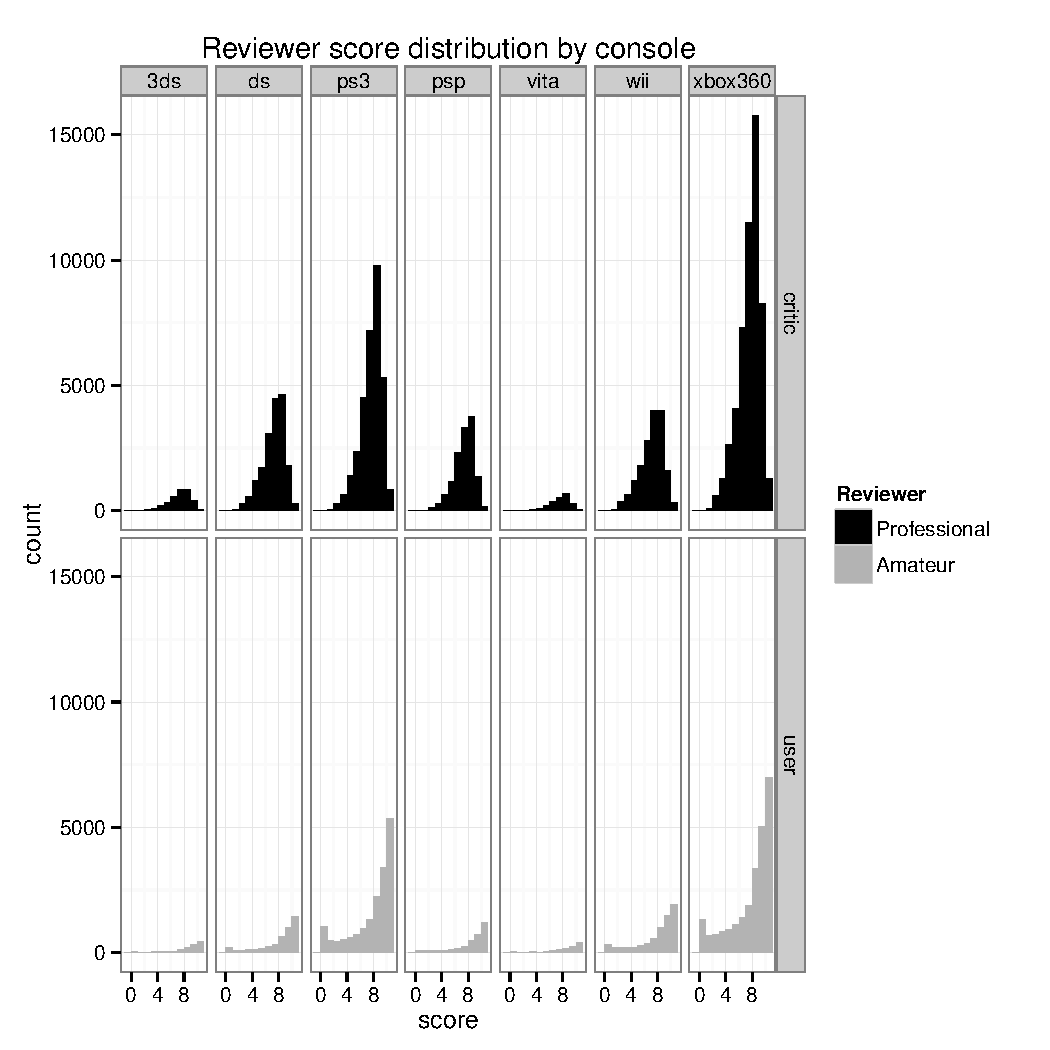
\includegraphics[width=\linewidth]{./console_reviews_score_hist}
%\caption{review score distribution by console}

% % for each review
%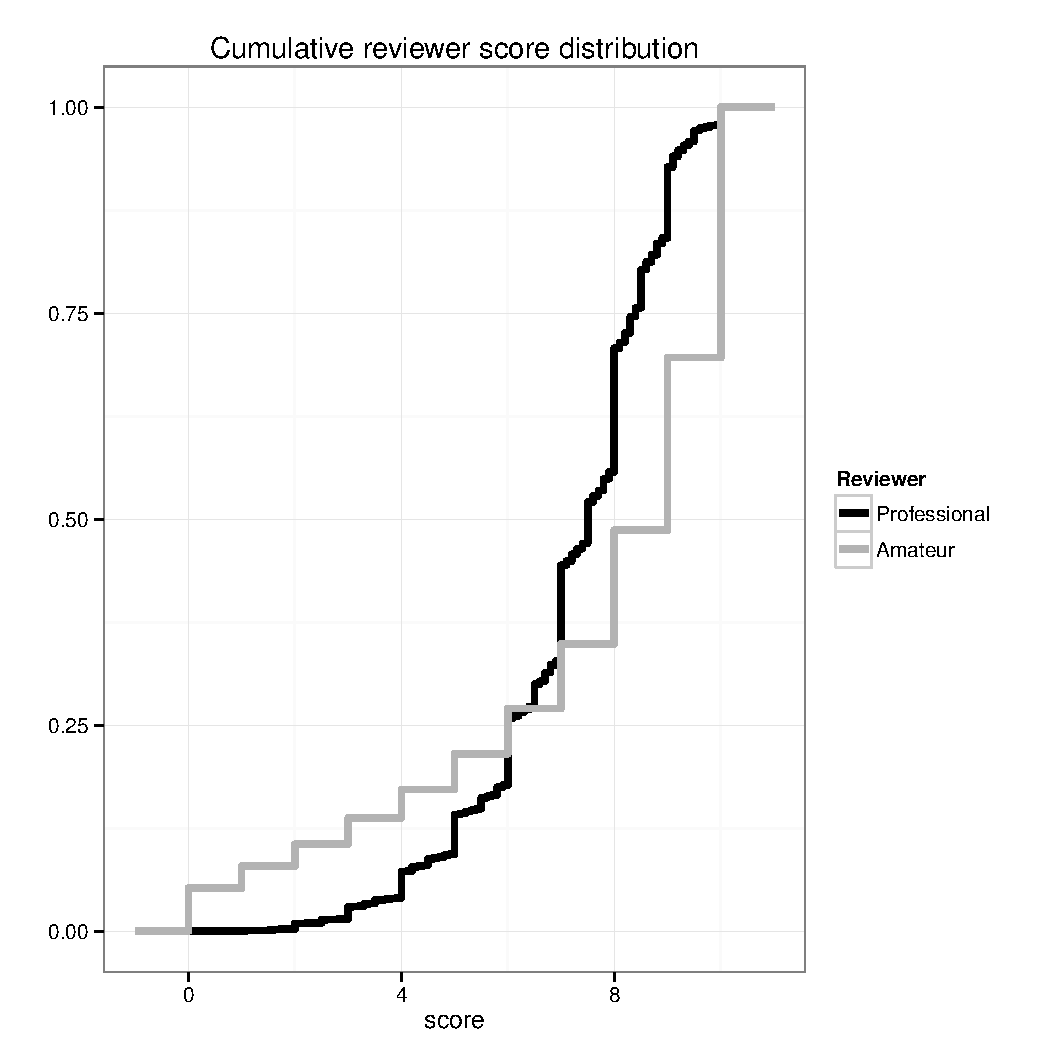
\includegraphics[width=\linewidth]{./console_reviews_score_ecdf}
%\caption{Cumulative review score distribution}

% % for each game
\begin{subfigure}[b]{\linewidth}
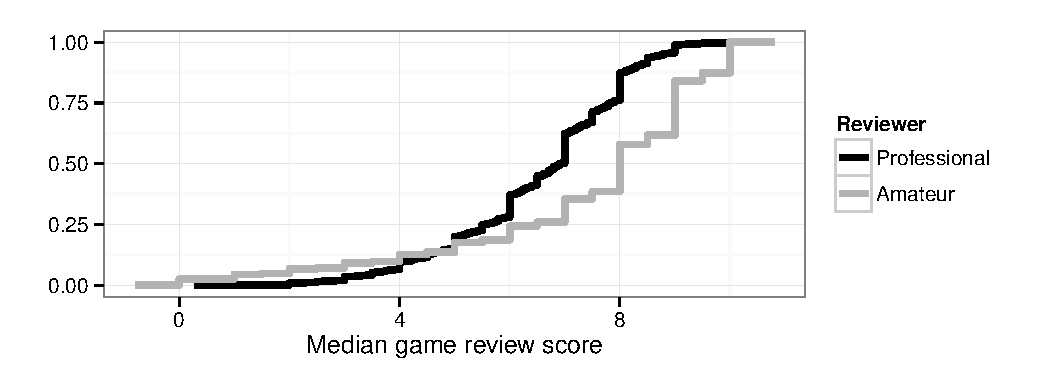
\includegraphics[width=\linewidth]{./console_games_scoremedian_ecdf}
\caption{Cumulative distribution of mean review score}
\label{fig:game_score}
\end{subfigure}
\begin{subfigure}[b]{\linewidth}
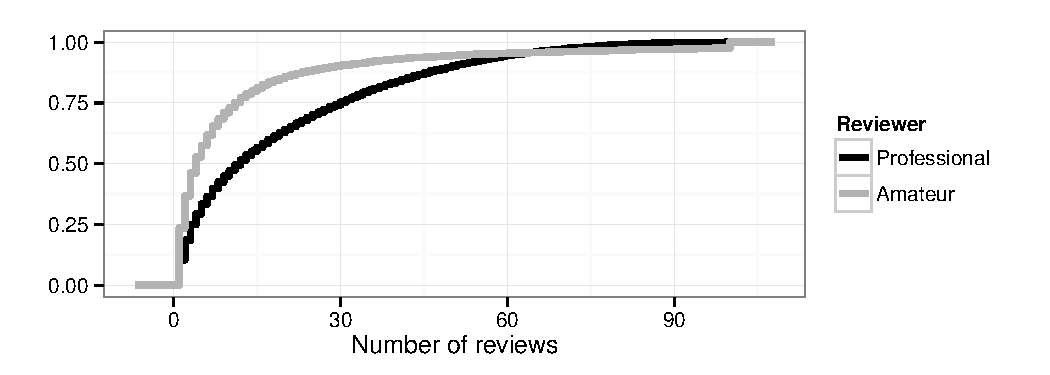
\includegraphics[width=\linewidth]{./console_games_numreviews_ecdf}
\caption{Cumulative distribution of number of reviews per game}
\label{fig:game_reviewnum}
\end{subfigure}
\caption{Game review corpus characteristics.}
\label{fig:revscore_console}
\end{figure}

\subsection{Review sentiment}
Reviewers and professionals show similar average levels of review sentiment, but differ in expressions of extreme sentiment (Figure \ref{fig:revsubj_density} and Table \ref{tab:review_pol_subj}).
For our analysis we considered both mean and median aggregations of
polarity and subjectivity features over all reviews; all results
reported were significant subject to a Wilcoxon test at p $< 0.001$, although these differences may not appear in Table \ref{tab:review_pol_subj} when rounding to two decimal places. While differences in mean and median per-review polarity and subjectivity were significant, their magnitude was small.
Both professionals' and amateurs' review distribution are slightly skewed toward more positive polarity and mild subjectivity (compare means and medians in Table \ref{tab:review_pol_subj}). 

Professionals and amateurs barely differ in mean polarity over a review, both centering on a mildly positive typical review. However, amateurs vary their sentence-level polarity more within reviews and show a strong skew towards at least one strongly positive and/or negative review sentence when compared to professionals (Figure \ref{fig:revpol_max}). Similarly, while professionals and amateurs show nearly the same level of moderate mean subjectivity, amateurs tend to use at least one highly subjective sentence (Figure \ref{fig:revsubj_max}). Interestingly, amateurs are also more likely to employ at least one highly \textit{objective} sentence, relating to their overall larger variance in expressions of subjectivity. Contrary to our expectations, professionals are not particularly objective when compared to amateurs, except in terms of the most polarizing and subjective sentences used in their reviews.

One limitation of this interpretation, however, is that professional
text was limited to summaries and thus may not reflect the intended valence of the review, but a revised summary meant to convey factual information for featuring on Metacritic. These results may also reflect limitations of our sentiment analysis and merit further investigation using full review text from the original review sites.

\begin{figure}[tb]
\centering

% % for each game aggregated
%\begin{subfigure}[b]{\linewidth}
%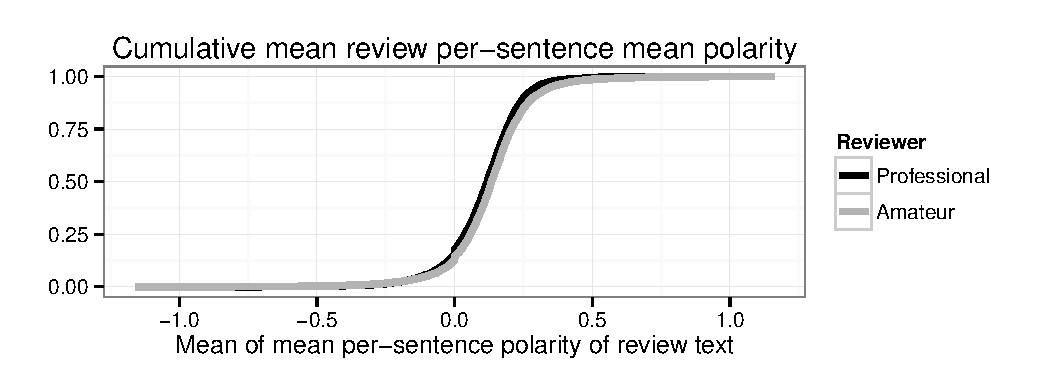
\includegraphics[width=\linewidth]{./console_games_polmeanmean_ecdf}
%\caption{Mean of mean per-sentence review polarity.}
%\label{fig:revpol_mean}
%\end{subfigure}
\begin{subfigure}[b]{\linewidth}
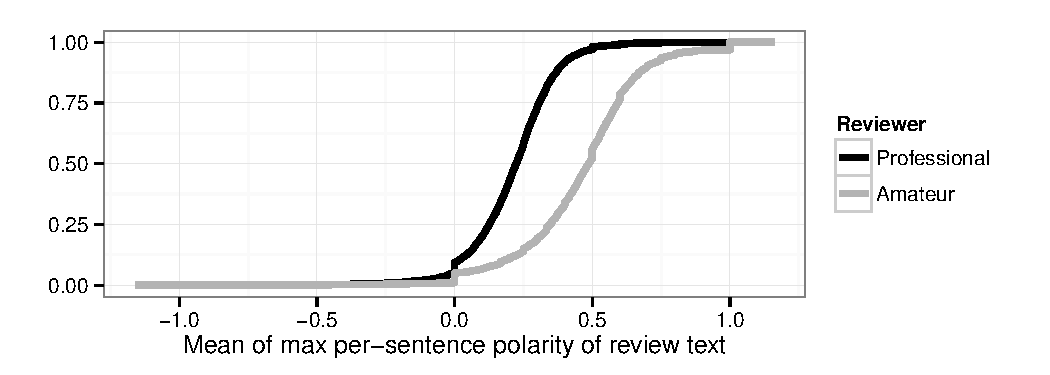
\includegraphics[width=\linewidth]{./console_games_polmaxmean_ecdf}
\caption{Cumulative distribution of mean of maximum per-sentence review polarity.}
\label{fig:revpol_max}
\end{subfigure}
%\caption{Cumulative review polarity distribution comparing reviewer type}
%\label{fig:revpol_density}

% % for each game aggregated
%\begin{subfigure}[b]{\linewidth}
%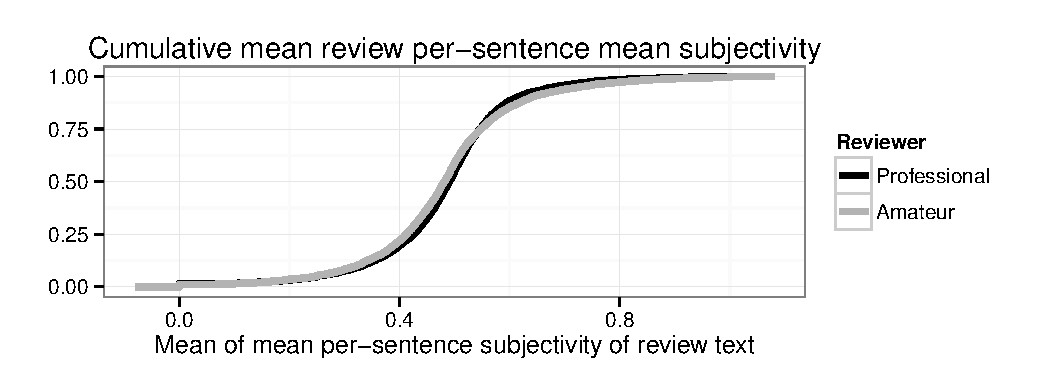
\includegraphics[width=\linewidth]{./console_games_subjmeanmean_ecdf}
%\caption{Mean of mean per-sentence review subjectivity.}
%\label{fig:revsubj_mean}
%\end{subfigure}
\begin{subfigure}[b]{\linewidth}
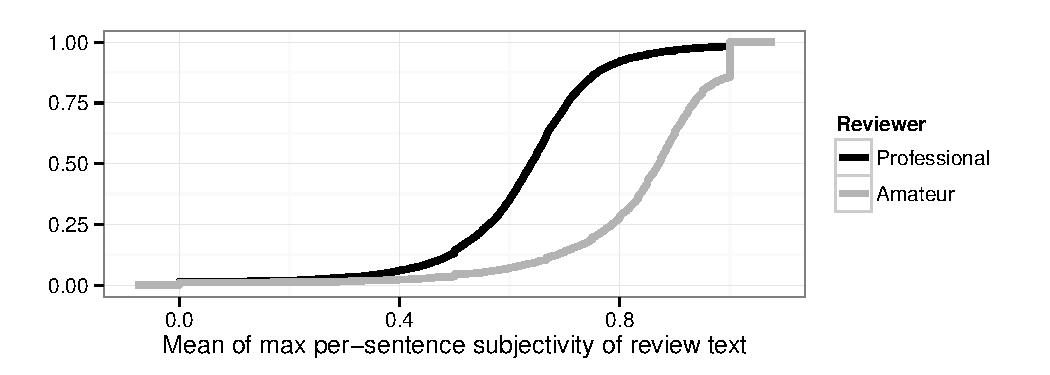
\includegraphics[width=\linewidth]{./console_games_subjmaxmean_ecdf}
\caption{Cumulative distribution of mean of maximum per-sentence review subjectivity.}
\label{fig:revsubj_max}
\end{subfigure}
\caption{Cumulative review sentiment (polarity and subjectivity) distributions comparing reviewer type}
\label{fig:revsubj_density}
\end{figure}


% % % separated polarity + subjectivity figures
%\begin{figure}[tb]
%\centering
%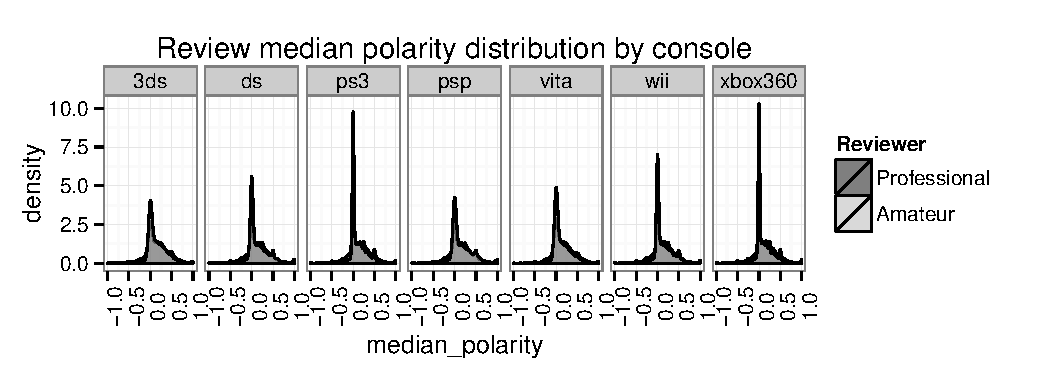
\includegraphics[width=\linewidth]{./console_reviews_polarity}
%\caption{review polarity density by console comparing reviewer type}

% % for each review
%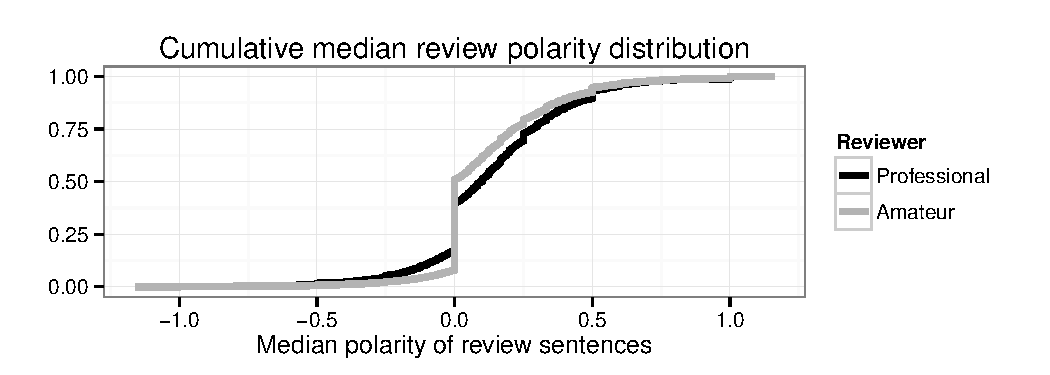
\includegraphics[width=\linewidth]{./console_reviews_polarity_ecdf}
%\caption{Cumulative review polarity distribution by console comparing reviewer type}

% % for each game aggregated
%\begin{subfigure}[b]{\linewidth}
%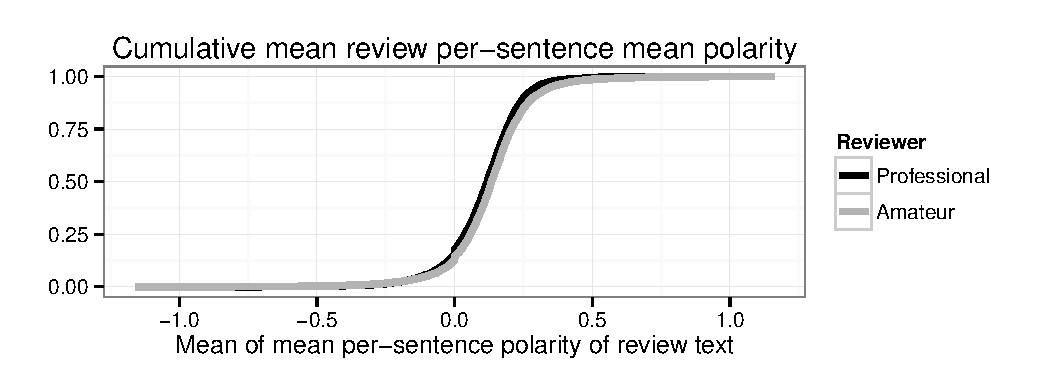
\includegraphics[width=\linewidth]{./console_games_polmeanmean_ecdf}
%\caption{Mean of mean per-sentence review polarity.}
%\label{fig:revpol_mean}
%\end{subfigure}
%\begin{subfigure}[b]{\linewidth}
%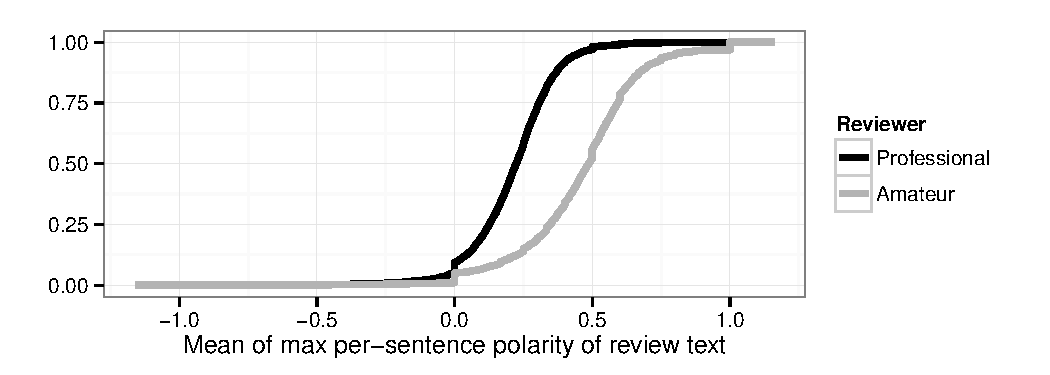
\includegraphics[width=\linewidth]{./console_games_polmaxmean_ecdf}
%\caption{Mean of maximum per-sentence review polarity.}
%\label{fig:revpol_max}
%\end{subfigure}
%\caption{Cumulative review polarity distribution comparing reviewer type}
%\label{fig:revpol_density}
%\end{figure}


%\begin{figure}[tb]
%\centering
%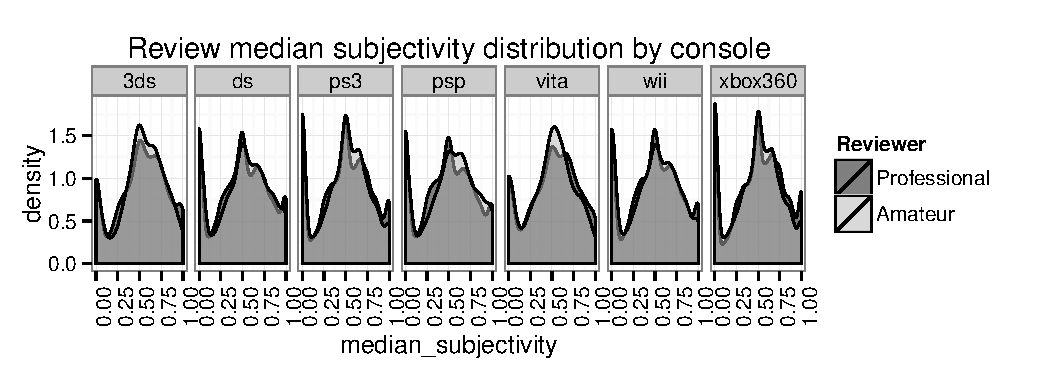
\includegraphics[width=\linewidth]{./console_reviews_subjectivity}
%\caption{review subjectivity density by console comparing reviewer type}

% % for each review
%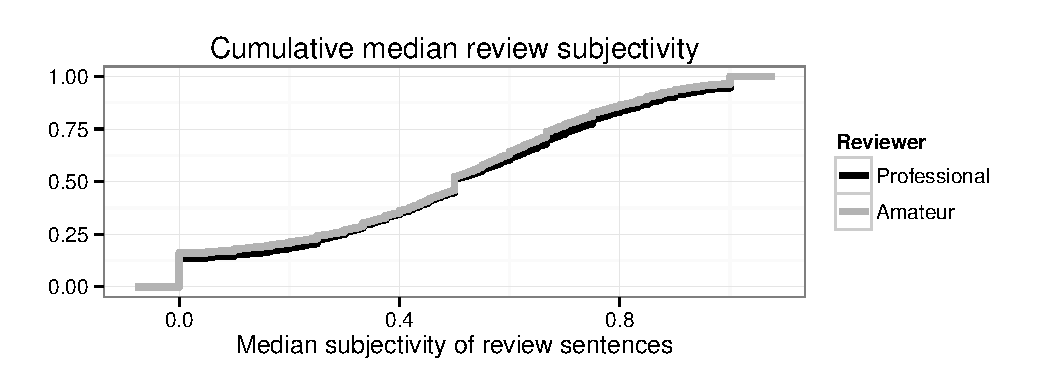
\includegraphics[width=\linewidth]{./console_reviews_subjectivity_ecdf}
%\caption{Cumulative review subjectivity distribution by console comparing reviewer type}

% % for each game aggregated
%\begin{subfigure}[b]{\linewidth}
%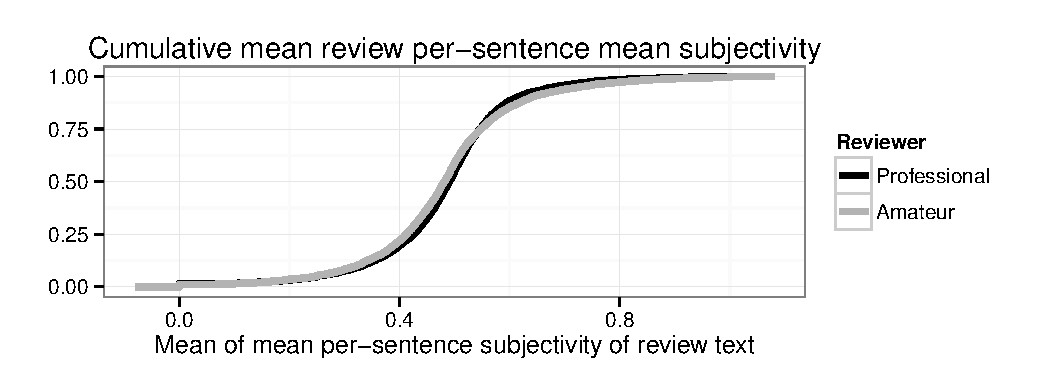
\includegraphics[width=\linewidth]{./console_games_subjmeanmean_ecdf}
%\caption{Mean of mean per-sentence review subjectivity.}
%\label{fig:revsubj_mean}
%\end{subfigure}
%\begin{subfigure}[b]{\linewidth}
%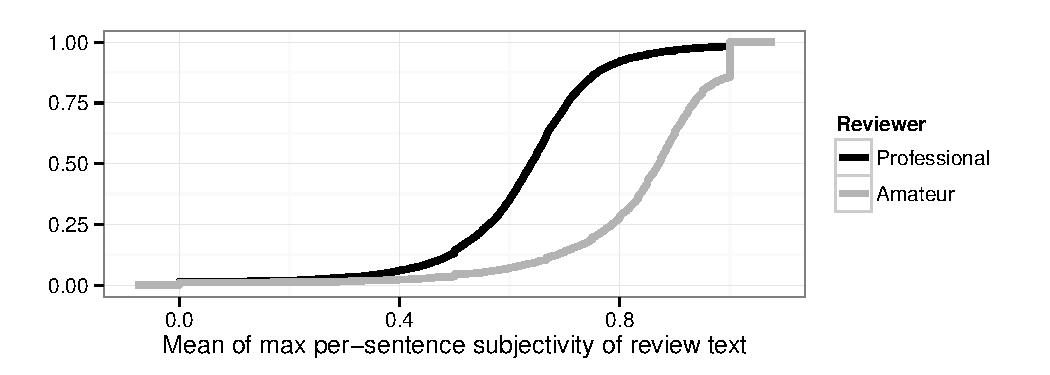
\includegraphics[width=\linewidth]{./console_games_subjmaxmean_ecdf}
%\caption{Mean of maximum per-sentence review subjectivity.}
%\label{fig:revsubj_max}
%\end{subfigure}
%\caption{Cumulative review subjectivity distribution comparing reviewer type}
%\label{fig:revsubj_density}
%\end{figure}


\subsection{Sales Prediction}
We used linear models to predict sales for each game, controlling for game console, genre, and Entertainment Software Rating Board (ESRB) maturity rating. While linear models may have limited predictive power for nonlinear relationships they afford direct interpretation useful to analysts employing the results. 

%We examined models for predicting game sales-to-date and net first ten week sales considering a set of factors: review author (professional or amateur), review scores, number of reviews, and review text features (length, polarity, subjectivity). 
We constructed four models: predicting total sales from reviews in the 10 weeks prior to the game's release (total vs pre-10), predicting net first 10 week sales from the same pre-release review subset (10 week vs pre-10), and predicting total sales using all reviews available with metascore, professional, and amateur score information (total vs meta). Table \ref{tab:regression_models} summarizes the models. Tables \ref{tab:sales_allmodel_lm} and \ref{tab:sales_metascore_lm} summarize the predictive variables, standardized $\beta$ coefficients, and model fitting results for each model.

\begin{figure}[tb]
\centering

\begin{subfigure}[b]{\linewidth}
\centering
% % raw scatterplot
%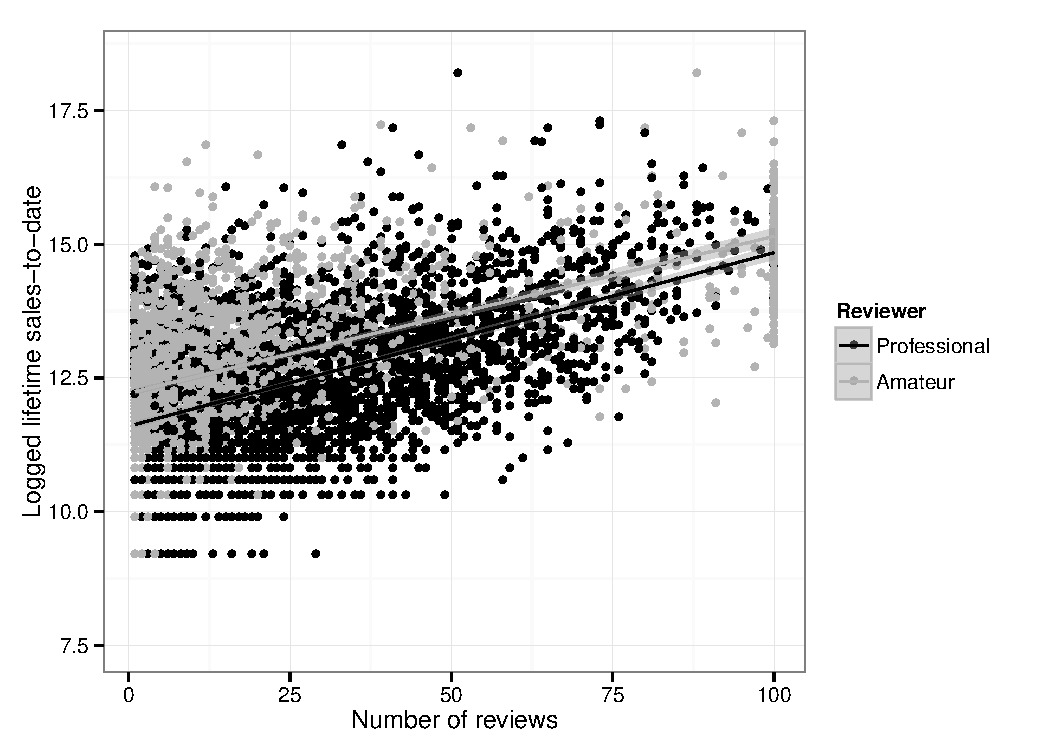
\includegraphics[width=\linewidth]{./sales_numscore_total}
%\caption{Lifetime sales-to-date vs number of reviews by reviewer type}

% % boxplot
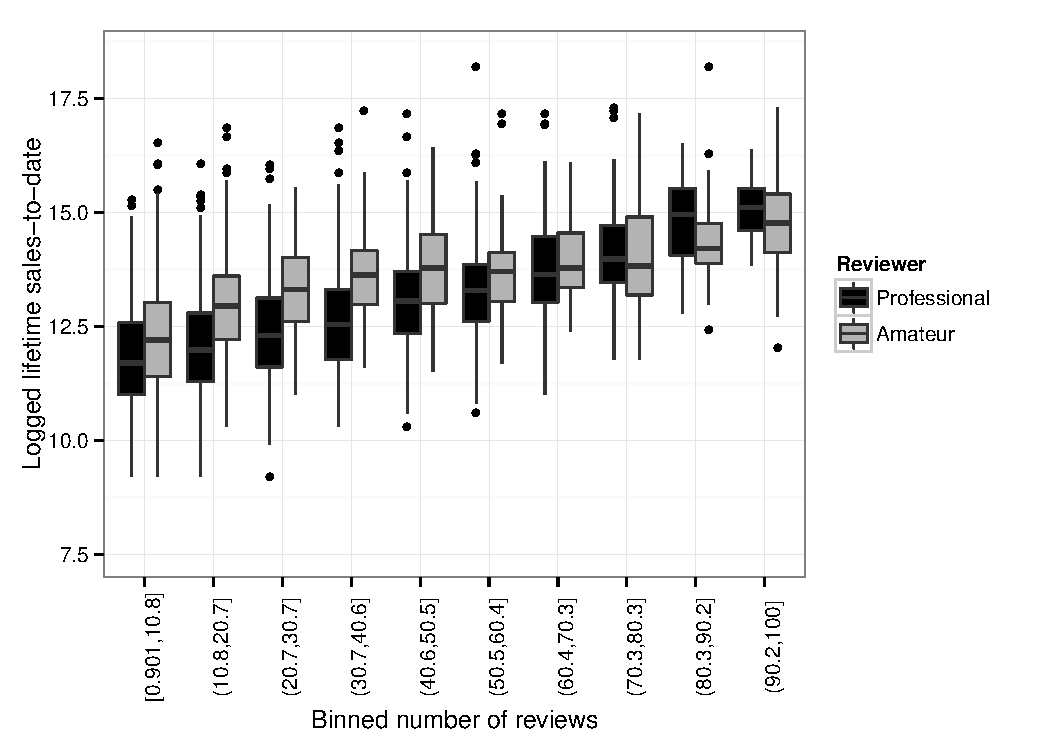
\includegraphics[width=\linewidth]{./sales_binnedct_vs_total}
\caption{Lifetime sales-to-date vs number of reviews by reviewer type}

% % 95\% confidence intervals
%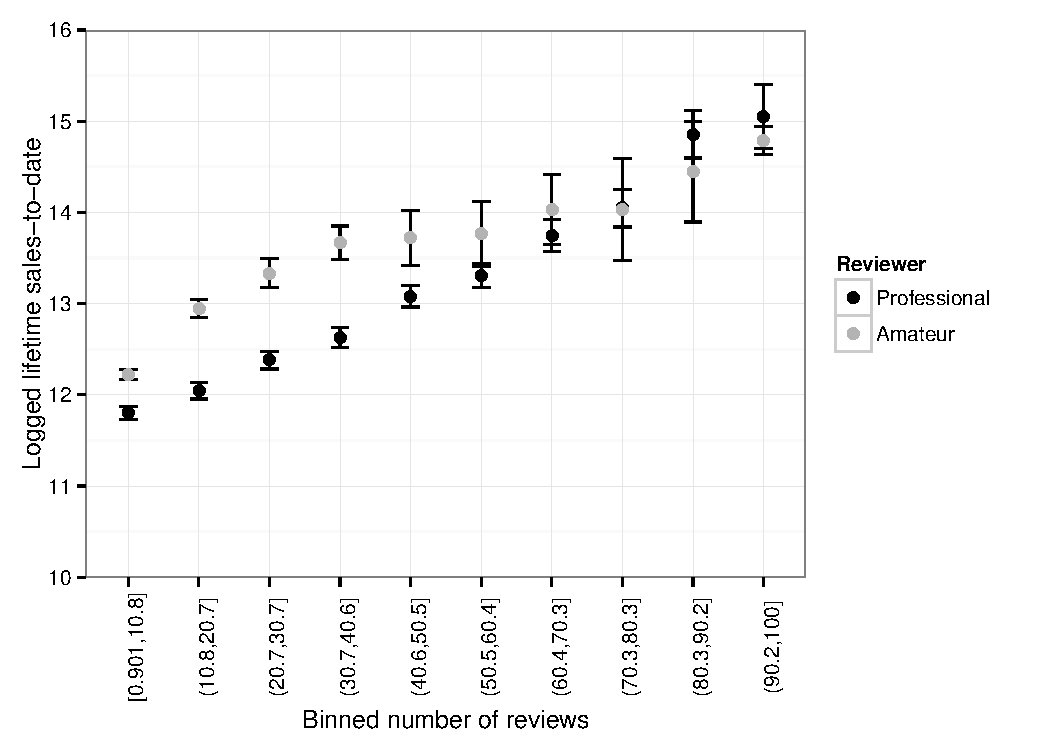
\includegraphics[width=\linewidth]{./sales_binnedct_vs_total_ci}
%\caption{Lifetime sales-to-date vs number of reviews by reviewer type}
\label{fig:lifesale_revnum}
\end{subfigure}

\begin{subfigure}[b]{\linewidth}
\centering
% % raw scatterplot
%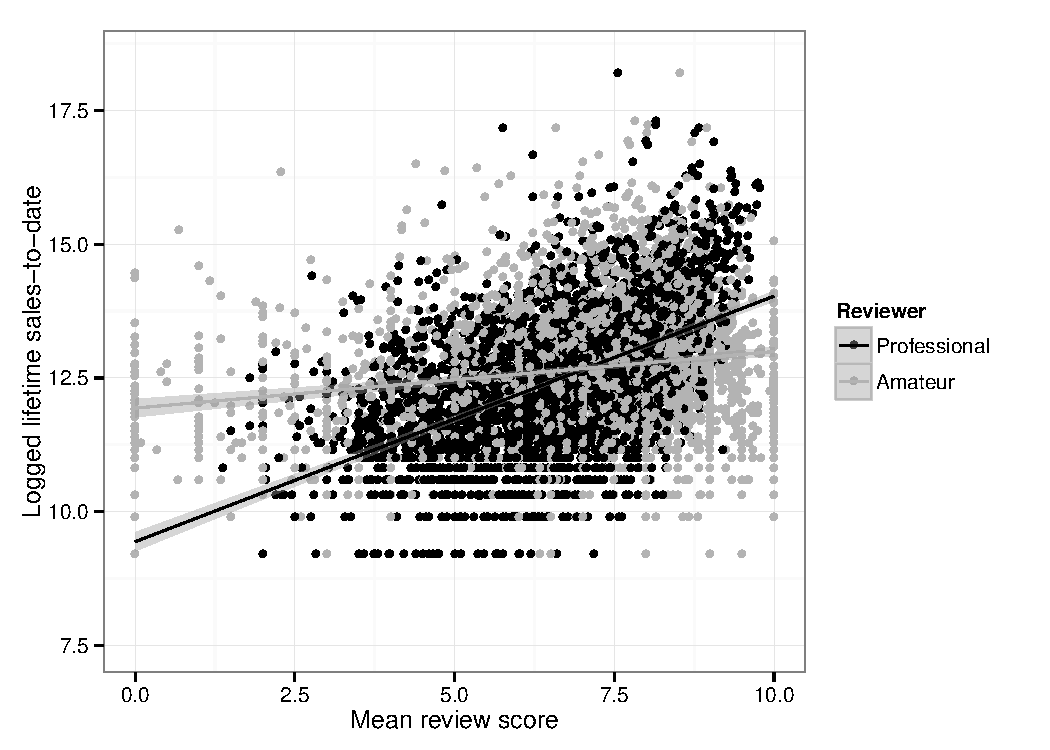
\includegraphics[width=\linewidth]{./sales_meanscore_total}
%\caption{Lifetime sales-to-date vs median review score by reviewer type}

% % boxplot
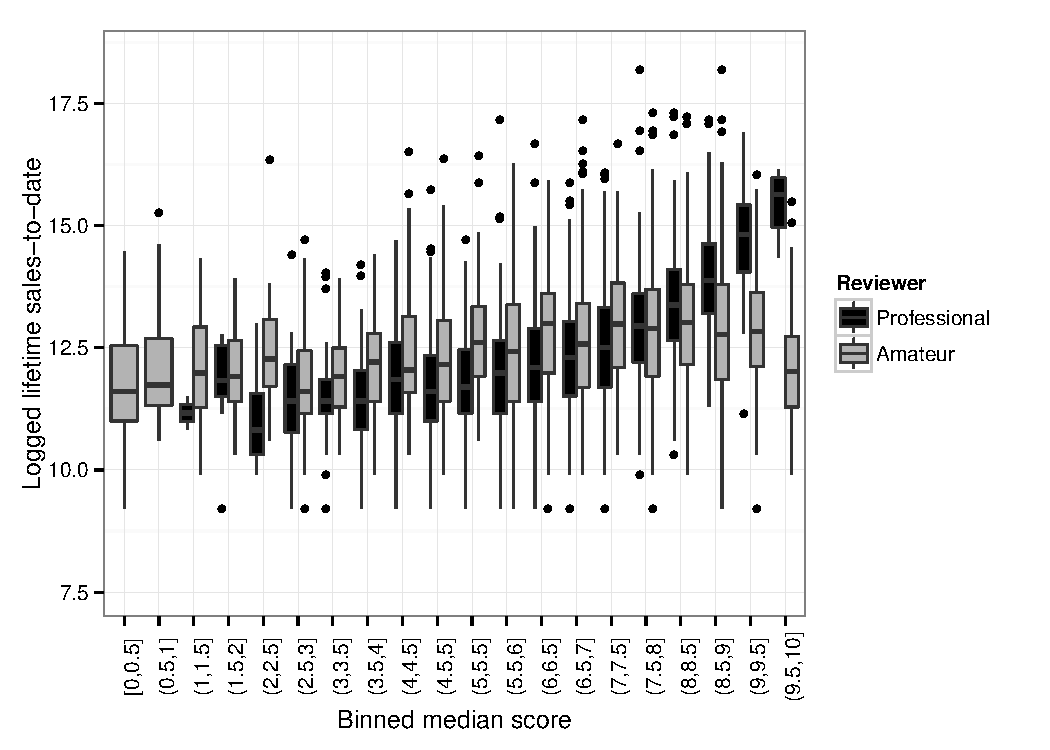
\includegraphics[width=\linewidth]{./sales_binnedscore_vs_total}
\caption{Lifetime sales-to-date vs mean review score by reviewer type}

% % 95\% confidence intervals
%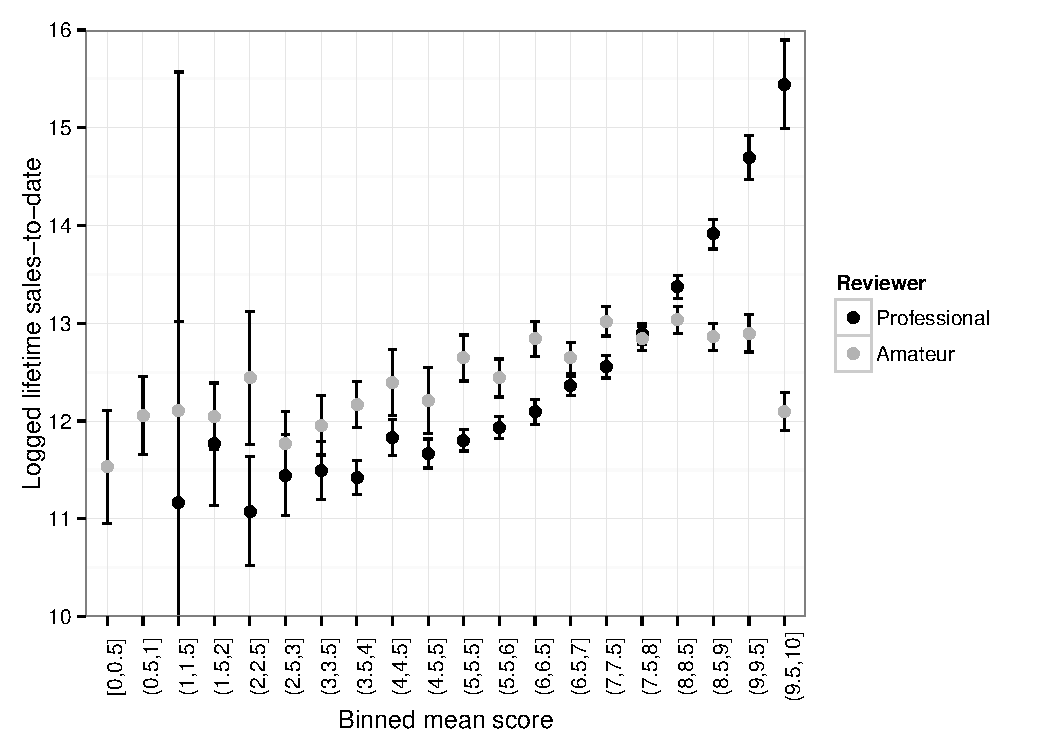
\includegraphics[width=\linewidth]{./sales_binnedscore_vs_total_ci}
%\caption{Lifetime sales-to-date vs mean review score by reviewer type}
\label{fig:lifesale_revscore}
\end{subfigure}

%\caption{Lifetime sales to date vs review scores and volume.}
%\caption{Mean lifetime sales-to-date (with 95\% confidence intervals) vs review scores and volume.}
\caption{Mean lifetime sales-to-date vs review scores and volume.}
\label{fig:lifesale_plots}
\end{figure}


Review scores and volume both show clear relationships to the lifetime sales of a game (Figures \ref{fig:lifesale_revnum} and \ref{fig:lifesale_revscore}). Anecdotally, many have claimed that a metascore over 90 (9 on our rescaled range) leads to a substantial boost to game sales. Our data supports this claim when considering aggregated professional scores, although the range of relevance is broader.\footnote{We found similar trends when examining Metascores, although the dataset is limited to fewer games.} Amateur scores do not show a clear relationship to sales: increasing mean amateur review score does not appear to relate to any substantial gain in scores. By contrast, professional review scores show a clear increasing relationship, starting around scores above 60 but becoming most prominent for scores above 80. While the [95-100] category has only 25 professional reviews and thus is of dubious predictive value, the [85-90] and [90-95] categories consist of 371 and 56 reviews and thus are of greater predictive merit.

\subsubsection{Prediction Models}
Our models show moderately strong predictive power ($R^2$ between $0.360$ and $0.446$, MSE between $0.669$ and $0.586$) for logged sales using standardized variables (Tables \ref{tab:sales_allmodel_lm} and \ref{tab:sales_metascore_lm}). Regression results report only standardized $\beta$ coefficients significantly different from 0 ($p < 0.001$); ``n.s.'' indicates non-significant coefficients. In all cases test models had a statistically significantly ($\chi^2$ test, $p < 0.001$) smaller deviance than control models that accounted for game console, genre, and ESRB rating. Thus, all models explain variance in game sales not accounted for game market factors, showing the predictive value of Metacritic amateur and professional reviews.

For each predictive task we computed all possible linear models formed from subsets of review score and text features and scored them according to the Bayesian Information Criterion (BIC) using R's leaps package.\footnote{http://cran.r-project.org/web/packages/leaps} Using the BIC allows our model selection process to penalize overly complex models to reduce the likelihood of overfitting. Relative importance of model features was measured using the lmg metric in R's relaimpo package.\footnote{http://cran.r-project.org/web/packages/relaimpo} The lmg metric calculates the average $R^2$ contribution of a feature averaged over orderings among predictive variables---we use relative values among predictors to compare their importance.


%\subsubsection{Total sales vs all reviews}
%\todo[inline]{should I cut this and just let the comparison in the metascore section handle this? qualitatively same results and this model isn't usefully ``predictive'' as it uses all of time}
% % yes, yes I should...
%For total sales we examined a model treating professional and amateur reviews as separate sources of predictors, looking only at games with data from both groups and using all reviews in our dataset (6809 games). The BIC identified the following variables (standardized $\beta$ coefficients are reported in parenthesis): mean professional review score (0.244), mean amateur review score (-0.038), number of professional reviews (0.309), number of amateur reviews (0.343), median of per-review maximum subjectivity from professional reviews (-0.044), mean of the same from amateur reviews (-0.030). Overall the model's adjusted $R^2$ value of $0.405$ and MSE of $0.600$ suggests a strong correlation between these factors and lifetime sales.
%We compared this model against those ablating one or more of the predictive variables and found the differences significant according to an ANOVA ($p < 0.05$), confirming this model includes only statistically meaningful variables.

% % from total sales prediction from all reviews
%\begin{table}[tb]
%\centering
%\scriptsize
%\begin{tabularx}{\linewidth}{|X|c|c|}
%\hline  & \multicolumn{2}{|c|}{\textbf{total vs all}}\\ 
%\hline \textbf{variable} & \textbf{$\beta$} & \textbf{relative importance}\\ 
%\hline mean professional score & 0.244411 & 23.23\%\\ 
%\hline mean amateur score & -0.038349 & 2.01\%\\ 
%\hline number professional reviews & 0.308787 & 25.08\%\\ 
%\hline number amateur reviews & 0.343262 & 30.86\%\\  
%\hline median(max review subjectivity) professionals & -0.044488 & 0.50\%\\ 
%\hline median(max review subjectivity) amateurs & -0.030322 & 0.18\%\\ 
%\hline 
%\end{tabularx}
%\caption{Regression models for lifetime sales-to-date using all available reviews. $\beta$ are standardized regression coefficients when predicting log-scaled and standardized lifetime sales. All values are significant at $p < 0.001$. \textbf{MAY CUT THIS ANALYSIS ALTOGETHER + replace w/comparing on only subset of metascore games}}
%\label{tab:sales_totsale_lm}
%\end{table}

%\todo[inline]{of control variables, esrb is always significant, as is platform, sometimes genre}
%\begin{table}[tb]
%\centering
%\scriptsize
%\begin{tabularx}{\linewidth}{|X|c|c|}
%\hline  & \multicolumn{2}{|X|}{\textbf{total vs all reviews} ($R^2 = 0.4053$, $MSE = 0.59995$)}\\ 
%\hline \textbf{variable} & \textbf{$\beta$} & \textbf{relative importance}\\ 
%\hline median score & 0.30145 & 15.80\%\\ 
%\hline number of reviews & 0.53365 & 53.32\%\\ 
%\hline reviewer type (as amateur) & 0.37623 & 4.79\%\\ 
%\hline reviewer type (as amateur) X median score & -0.21179 & 2.60\%\\  
%\hline reviewer type (as amateur) X mean(mean review polarity) & 0.03635 & 2.31\%\\ 
%\hline reviewer type (as professional) X mean(mean review subjectivity) & -0.02785 & 0.17\%\\ 
%\hline 
%\end{tabularx}
%\caption{Regression model for lifetime sales-to-date comparing metascores, amateurs, and professionals. $\beta$ are standardized regression coefficients when predicting log-scaled and standardized lifetime sales. All values are significant at $p < 0.001$ except median(median review subjectivity) which is marginally significant at $p < 0.1$.}
%\label{tab:sales_allreview_lm}
%\end{table}

%As expected from the previous distributions, review subjectivity is a weak factor for predicting total sales. Sheer volume of amateur and professional reviews account for the largest part of our model's power. Intuitively this makes sense: volume of professional and amateur reviews both reflect relative attention to a game and also likely reflect the relative publishing and marketing resources behind the game's developer. More amateur reviews reflect games more people have played and thus likely already purchased. Further, games that drive amateurs to respond on online forums reflect greater social popularity. A greater volume of professional reception similarly reflects publisher budget and expectations. Review copies are typically distributed to professionals when publishers expect games to be reviewed well, bolstering their review numbers. Further, only more well-financed and established publishers are able to push their games to be reviewed by venues that Metacritic would index and report from.

%While professional scores and number of reviews have roughly equal relative importance, amateur scores are relatively unimportant. Given the distributions seen above this makes sense: games that have many amateur reviews are rare, but enjoy strong sales on average. For a game to have many amateur reviews requires many amateurs to have played the game and been motivated to review the game. From the previous distributions of review scores we would expect these reviewers to (mostly) give positive scores, thus the fact that they are writing a score at all is indicative of what that score will be. Playing the game typically means a amateur has purchased the game, thus further entangling with sales. While direct causality cannot be read off from these results it is clear that the amount of attention amateurs or professionals devote to a game is indicative of its level of sales success. Future work should explore more sophisticated features for predicting sales such as volume of previews, media campaign efforts, and user interested expressed on Twitter, Facebook, Youtube and other media outlets. These sources may provide complimentary information on more broad interest in a product compared to those devoted enough to use Metacritic as a review outlet.


\subsubsection{Total and net 10 week sales vs pre-release reviews}
Marketers often seek to predict sales for unreleased games relying solely on information available prior to a game's release. For this application, we examined two models that used reviews only in the 10 weeks prior to the release of a game to predict either lifetime sales-to-date or net sales over the first 10 weeks after a game releases.

The BIC identified the following predictive features: median review score, number of reviews, type of review (amateur or professional), and interactions between type of reviewer and median score, number of reviews, mean of mean per-sentence review polarity and mean of mean per-sentence review subjectivity.
%Due to the sparsity of games that possessed either professional and amateur reviews in this period (600 total) we used the same predictive features as above but with a dummy variable indicating reviewer type (professional or amateur) and adding terms to assess interaction effects between this variable and the other predictors (scores and sentiment). For example, rather than examine how mean professional scores impact sales we instead examine how scores impact sales and how this relationship is mediated by the type of reviewer providing the score. 
With an adjusted $R^2$ of $0.360$ and MSE of $0.669$ the pre-release review model is moderately effective at predicting lifetime sales. Table \ref{tab:regression_models} shows the slightly better performance of the pre-release review model when predicting first 10 week sales. This is not surprising as most game sales occur during the initial launch and marketing period, with relatively few games having more long-term strong sales or shifts in sales. In this dataset, net first 10 week sales and total lifetime sales-to-date have a Spearman's rank correlation coefficient of 0.849, confirming this relationship.

We compared these models with a third model that employed all reviews (rather than solely pre-release reviews) for predicting total sales (``total vs all''); this model covered 2902 games, rather than the 600 in the previous models. Using all reviews gives an upper bound on performance for sales prediction given the information in our reviews, at least as we have processed it. All three models for sales prediction considering review features and their interactions with reviewer types show qualitatively similar effects (Table \ref{tab:sales_allmodel_lm}). 

In general, number of reviews is most important for sales prediction, followed by median review score, and the interaction between median review score and reviewer type. Review sentiment factors are less important and have smaller coefficients in most cases. These three aspects account for most of these models' predictive power. Median review scores have the most positive effect on sales with the interaction of these scores with reviewers as amateurs being equally powerful but \textit{negative}. Higher scores suggest strong sales, but not when coming from amateurs, who tend to provide the same scores across games of varying commercial success. Number of reviews has a weaker positive effect than review scores. Together these results show professional scores and review volume indicate positive critical reception, while amateur reviews are only useful as a gauge of popular interest.

%\todo[inline]{more integration or potentially cut---more of a ``discussion'' than results}
%Sheer volume of amateur and professional reviews account for the largest part of our model's power. Intuitively this makes sense: volume of professional and amateur reviews both reflect relative attention to a game and also likely reflect the relative publishing and marketing resources behind the game's developer. More amateur reviews reflect games more people have played and thus likely already purchased. Further, games that drive amateurs to respond on online forums reflect greater social popularity. A greater volume of professional reception similarly reflects publisher budget and expectations. Review copies are typically distributed to professionals when publishers expect games to be reviewed well, bolstering their review numbers. Further, only more well-financed and established publishers are able to push their games to be reviewed by venues that Metacritic would index and report from.

%While professional scores and number of reviews have roughly equal relative importance, amateur scores are relatively unimportant. Given the distributions seen above this makes sense: games that have many amateur reviews are rare, but enjoy strong sales on average. For a game to have many amateur reviews requires many amateurs to have played the game and been motivated to review the game. From the previous distributions of review scores we would expect these reviewers to (mostly) give positive scores, thus the fact that they are writing a score at all is indicative of what that score will be. Playing the game typically means a amateur has purchased the game, thus further entangling with sales. 

Volume of professional and amateur reviews both reflect relative attention to a game and the relative publishing and marketing resources backing the game's developer. More amateur reviews reflect more people have played a game and thus likely already purchased it.
More professional reviews likely reflect publisher budget and expectations. Review copies are typically distributed to professionals when publishers expect games to be reviewed well, bolstering their review numbers. Further, only more well-financed and established publishers are able to push their games to be reviewed by venues that Metacritic would index and report from.

While direct causality cannot be read off from these results it is clear the amount of attention amateurs or professionals devote to a game relates to its sales success. Future work should explore more sophisticated features for predicting sales such as game previews, media campaigning, and interest expressed on Twitter, Facebook, Youtube and other media outlets. These sources may provide complimentary information on broader interest in a product compared to the narrower base of Metacritic reviewers.

%Directionally these results have the same message: volume of reviews is most important, followed by receiving favorable review scores, with all other factors playing a relatively minor role. Knowing amateurs are providing review scores lowers the estimated effect on sales while knowing more amateurs are writing reviews raises the estimate effect on sales. We created an analogous model predicting net sales over the first 10 weeks, achieving an adjusted $R^2$ of $0.306$ and MSE of $0.718$. Results were qualitatively the same as the total sale model, refer to Table \ref{tab:sales_allmodel_lm} for details. This is not surprising as most game sales occur during the initial launch and marketing period, with relatively few games having more long-term strong sales or shifts in sales.

%\begin{table*}[tb]
%\centering
%\scriptsize
%\begin{tabular}{|l|c|c|c|c|}
%\hline & \multicolumn{2}{|c|}{\textbf{10 week vs pre-10}} & \multicolumn{2}{|c|}{\textbf{total vs pre-10}}\\ 
%\hline \textbf{variable} & \textbf{$\beta$} & relative importance & \textbf{$\beta$} & relative importance\\ 
%\hline median review score & 0.64691 & 18.63\% & 0.553424 & 19.88\%\\ 
%\hline number of reviews & 0.23578 & 21.06\% & 0.235556 & 20.88\%\\ 
%\hline reviewer type (as amateur) & 0.43711 & 2.60\% & 0.606100 & 10.76\%\\ 
%\hline reviewer type (as amateur) X median score  & -0.61708 & 12.93\% & -0.505708 & 11.01\%\\ 
%\hline reviewer type (as amateur) X number of reviews & 0.51815 & 1.98\% & 0.431584 & 1.76\%\\ 
%\hline reviewer type (as amateur) X mean(mean review polarity) & 0.25741 & 4.70\% & 0.213716 & 4.50\%\\ 
%\hline reviewer type (as amateur) X mean(mean review subjectivity) & -0.20898 & 2.77\% & -0.170682 & 2.33\%\\ 
%\hline 
%\end{tabular}
%\caption{Regression models for lifetime sales-to-date and first 10 weeks net sales using reviewers in 10 weeks prior to game release. $\beta$ are standardized regression coefficients when predicting log-scaled and standardized lifetime sales. All values are significant at $p < 0.001$.}
%\label{tab:sales_prerelease_lm}
%\end{table*}

\begin{table*}[tb]
\centering
\small
\sffamily
\begin{tabular}{lllllll}
& \multicolumn{2}{c}{\textbf{10 week vs pre-10}} & \multicolumn{2}{c}{\textbf{total vs pre-10}} & \multicolumn{2}{c}{\textbf{total vs all}}\\ 
\midrule & \textbf{$\beta$} & rel. importance & \textbf{$\beta$} & rel.
importance & \textbf{$\beta$} & rel. importance\\ 
median review score & 0.64691 & 18.63\% & 0.553424 & 19.88\% & 0.30145 & 15.80\%\\ 
number of reviews & 0.23578 & 21.06\% & 0.235556 & 20.88\% & 0.53365 & 53.32\%\\ 
is amateur & 0.43711 & 2.60\% & 0.606100 & 10.76\% & 0.37623 & 4.79\%\\ 
is amateur x median score  & -0.61708 & 12.93\% & -0.505708 & 11.01\% & -0.21179 & 2.60\%\\  
is amateur x number of reviews & 0.51815 & 1.98\% & 0.431584 & 1.76\% & n.s. & n.s. \\ 
is amateur x mean review polarity & 0.25741 & 4.70\% & 0.213716 & 4.50\% & 0.03635 & 2.31\%\\ 
is amateur x mean review subjectivity & -0.20898 & 2.77\% & -0.170682 & 2.33\% & -0.02785 & 0.17\%\\ 

\end{tabular}
\caption{Regression models for lifetime sales-to-date and first 10 weeks net sales. $\beta$ are standardized regression coefficients when predicting log-scaled and standardized lifetime sales. All values are significant at $p < 0.001$.}
\label{tab:sales_allmodel_lm}
\end{table*}

%\hline median score & 0.30145 & 15.80\%\\ 
%\hline number of reviews & 0.53365 & 53.32\%\\ 
%\hline reviewer type (as amateur) & 0.37623 & 4.79\%\\ 
%\hline reviewer type (as amateur) X median score & -0.21179 & 2.60\%\\  
%\hline reviewer type (as amateur) X mean(mean review polarity) & 0.03635 & 2.31\%\\ 
%\hline reviewer type (as professional) X mean(mean review subjectivity) & -0.02785 & 0.17\%\\ 

\subsubsection{Comparing Metascores, professionals, and amateurs}
To better understand the efficacy of different scoring systems we compared the predictive power of metascores, combined professional review scores, and combined amateur scores for predicting lifetime sales-to-date. From the total dataset, 840 games have data on lifetime sales-to-date, metascores, and reviews from both professionals and reviews. We predict lifetime sales as metascores are running values that are updated without a historical trace---thus we cannot know historical values of metascores prior to a game's launch. Professional and amateur reviews were aggregated across the full set of data for a fair comparison with metascores.

According to the BIC criteria the best linear model (adjusted $R^2 = 0.4457$, MSE $= 0.586$) uses (standardized $\beta$ in parenthesis): metascores (0.449), median professional scores (-0.093), median amateur scores (-0.190), and number of professional reviews (0.282) (Table \ref{tab:sales_metascore_lm}). Removing metascore information shifts the model to positively weight amateur review scores (0.223) and add number of amateur reviews (0.235) as a significant predictive factor. The model without metascores is a somewhat worse fit ($R^2 = 0.4298$, and MSE $= 0.599$) according to a $\chi^2$ test ($p < 0.001$).

As in the previous models, volume of amateur and professional reviews captures a large portion of the model's predictive power, using metascores for score information. The small differences in model fit suggest metascores are no more predictive than amateur or professional scores combined by simple weighting schemes (mean or median). 

That amateur scores were not predictive of sales when coupled to metascores surprised us. To understand this effect we examined the Spearman's rank correlation between metascores, amateur scores, and professional scores. Surprisingly, metascores are very strongly correlated with median amateur scores ($\rho = 0.978$) and more weakly correlated with median professional reviews ($\rho = 0.545$). The comparable overall model power between using only amateur and professional data for lifetime sales and adding metascores suggests the metascore weighting scheme may not be particularly powerful compared to simpler methods.

\begin{table}[tb]
\centering
\small
\sffamily

%\begin{tabularx}{\linewidth}{|c|c|X|c|X|}
%\hline  & \multicolumn{2}{|c|}{\textbf{with Metascores}} & \multicolumn{2}{|c|}{\textbf{no Metascores}}\\ 
%\hline \textbf{variable} & \textbf{$\beta$} & \textbf{rel. imp.} & \textbf{$\beta$} & \textbf{rel. imp.}\\ 
%\hline metascore & 0.386 & 11.07\% & - & - \\ 
%\hline mean professional score & -0.071 & 1.61\% & -0.051 & 1.7\% \\ 
%\hline mean amateur score & n.s. & 8.93\% & 0.222 & 16.47\% \\ 
%\hline number reviews in metascore & n.s. & 12.53\% & - & - \\ 
%\hline number professional reviews & 0.280 & 21.58\% & 0.273 & 27.93\% \\ 
%\hline number amateur reviews & n.s. & 12.64\% & 0.229 & 22.18\% \\ 
%\hline 
%\end{tabularx}

\begin{tabularx}{\linewidth}{llXlX}
& \multicolumn{2}{c}{\textbf{with metascores}} & \multicolumn{2}{c}{\textbf{no metascores}}\\ 
\midrule & \textbf{$\beta$} & imp. & \textbf{$\beta$} & imp.\\ 
metascore & 0.449 & 11.49\% & - & - \\ 
median professional score & -0.093 & 1.87\% & -0.071 & 1.90\% \\ 
median amateur score & -0.190 & 8.51\% & 0.223 & 15.68\% \\ 
number reviews in metascore & n.s. & 12.51\% & - & - \\ 
number professional reviews & 0.282 & 21.60\% & 0.280 & 28.28\% \\ 
number amateur reviews & n.s. & 12.62\% & 0.235 & 22.48\% \\ 

\end{tabularx}
\caption{Regression model for lifetime sales-to-date comparing metascores, amateurs, and professionals. $\beta$ are standardized regression coefficients when predicting log-scaled and standardized lifetime sales. All values not listed as not significant (``n.s.'') are significant at $p < 0.05$. 
% % mean model
%Model $R^2 = 0.4420$, $MSE = 0.58995$ when including Metascores, $R^2 = 0.4297$, $MSE = 0.59879$ without. 
%Metascore model is significantly different from null model (residual deviance 468 on 816 degrees of freedom, null deviance 839 on 838 degrees of freedom, $\chi^2$ test $p < 0.001$). Model without Metascore is also (residual deviance 478 on 818 degrees of freedom, null deviance 838 on 838 degrees of freedom, $\chi^2$ test $p < 0.001$). $chi^2$ test finds two models significantly different at $p < 0.001$.
% % median model
With metascores, the model has $R^2 = 0.4457$ and $MSE = 0.586$; without metascores has $R^2 = 0.4298$ and $MSE = 0.599$. 
The metascore model is significantly different from the null model (residual deviance 465 on 816 degrees of freedom, null deviance 839 on 838 degrees of freedom, $\chi^2$ test $p < 0.001$). The model without metascores is significantly different from both the null model (residual deviance 478 on 818 degrees of freedom, null deviance 838 on 838 degrees of freedom, $\chi^2$ test $p < 0.001$) and the model with metascores ($\chi^2$ test $p < 0.001$).
}
\label{tab:sales_metascore_lm}
\end{table}

%metascores have $\rho = 0.9607868$ with mean user scores, $\rho = 0.9615704$ with median user scores, but only $\rho = 0.5733836$ with mean critic and $0.5727746$ with median critic scores. So metascores are just as good as using amateur scores, hence why only one is used in the model.

%\subsubsection{ranking reviewers}
%no amateurs w/more than 10 reviews + strong sales correlation. some professionals negative correlation. subset of top gets prediction to $\approx 0.308$.
%\todo[inline]{review ``importance'' via score correlation; not needed for main story}


\section{Review Text Classification}
Our previous analyses show reviews are predictive of sales. But what
aspects of reviews distinguish them, particularly in terms of the words
used? We explored this question by using review text in a bag of words
model to classify reviewers as professionals or amateurs using a
penalized binomial regression model. Understanding these text-level
differences can enable better prediction of what characteristics
distinguish professional reviews in content from amateur reviews.

The model achieved an F1 score of $0.9359$ (precision $90.96\%$ and
recall $96.38\%$) over the set of 197,383 reviews for which we had data. $96.38\%$ of professionals were correctly labeled, and $77.28\%$ of amateurs were correctly labeled, reflecting the imbalanced proportions of these categories in our data set---$70.34\%$ of reviews come from professionals, $29.66\%$ from amateurs. 10-fold cross-validation found the model had a MSE of 0.4980. The penalized regression model employed 2,570 terms, assigning 146 a weight of zero, 1,235 positive weights (being an amateur), and 1,190 negative weights (being a professional). 

Below we examine several of the terms from these groups to understand how amateurs and professionals differentiate themselves in text descriptions with term coefficients in parenthesis. As words were stemmed we included completions of the stems in parentheses to help interpretation. Table \ref{tab:user_classification_coef} illustrates a selection of words with strong predictive power: $\beta$ coefficients are reported in parentheses with positive values predicting a reviewer to be a amateur. Word categories were derived through inspection and are not part of the predictive model, but shown to highlight trends in how amateurs and professionals word their reviews. 

Professionals were most recognizable by references to major game genres and the games market. Compared to amateurs, professionals are more likely to mention words linking a game to marketing and game industry competition, using terms such as ``tie(-)in'' (-1.53) and ``competitor'' (-1.44). References to game genres included descriptions of gameplay perspective---``firstperson'' (-0.86) and ``thirdperson'' (-1.01)---as well as gameplay style--``action'' (0.36), ``roleplay'' (-1.34),  and ``brawler'' (-0.78). Professional reviews often characterize a game within the broader industry sales cycle and specific genres of interest. This makes intuitive sense---professional reviews are often a form of marketing for companies, acting to define the intended audience of a game through describing how it relates to a broader marketing strategy and genre. Professionals more often refer to game features and the demographics of players who may be interested for these reasons.

Amateurs were recognizable by slang terms, references to game purchasing and reviewing, family, multiplayer, and aspects of the running game. Slang terms included phrases such as ``wtf'' (2.32), ``imo'' (4.59), ``lol'' (2.77), and ``meh'' (1.20). Reviews often mentioned aspects of reviewing games through references to review websites and aspects of ``bias'' (2.45) and ``opinion'' (1.46). Game purchasing appeared through game pricing, purchase options, and places to purchase games (e.g., the ``Gamestop'' (3.31) retail chain). Amateurs often reference the social dynamics of play, mentioning family and multiplayer as well as problems with actual game bugs or flaws. Mentioning live gameplay features and family members reflects amateurs' stronger emphasis on the experience of playing with others, rather than assessing a potential product for (implicitly individual) consumption as done in professional reviews.

%Terms removed from the model varied widely, covering topics that in some ways bridge the two reviewer groups. Several terms referenced games as franchises---``reboot'' and ``sequel''---while others noted target audiences---``child'' and ``adult''. ``Broken'' a term referring to dysfunctional gameplay seems to be shared across amateurs and professionals. Overall, however, there do not seem to be strong patterns among words not distinguishing the groups, suggesting these terms are simply a general vocabulary with relatively little significance for understanding game reviewing behavior.

Combined, these results paint a picture of professionals taking a role of identifying purchase products and describing their features, while amateurs relate their games to broader consumption practices and gaming culture. Amateurs are free to reference particular game distributors or review biases in ways professionals cannot. Compared to professionals, amateurs typically relate games back to playing behavior, experiences, and social interactions. In part these results help clarify the power of professional review scores to predict sales better than amateur review scores. Professionals describe games in a way to guide purchasing decisions, while amateurs are more likely to reflect on a game in their play practices and purchasing experiences while giving relatively little information on the game's features.

\begin{table}[tb!]
%\scriptsize
\centering
\small
\sffamily
%\begin{tabularx}{\linewidth}{|c|cc|}
\begin{tabular}{llc}
\textbf{category} & \textbf{word} & $\beta$ \\ 
\midrule 
game genre 
& roleplay & -1.34 \\
& thirdperson & -1.01 \\
%& firstperson &-0.86 \\
%& brawler & -0.78 \\
& openworld & -0.68 \\
& singleplay(er) & -0.67 \\
%& action(-)adventure & -0.61 \\
& oldschool & -0.47 \\
%& adventur(e) & -0.44 \\
%& strateg(y) & -0.42 \\ 
%& action & -0.36 \\
& sidescrol(ler) & -0.32 \\ [2ex]

\midrule 
game market 
& tie(-)in & -1.53 \\
& competitor & -1.44 \\ 
& holiday & -1.09 \\ 
& followup & -0.64 \\ 
& brand & -0.59 \\ 
%& predecessor & -0.50 \\ 
& publish & -0.41 \\ 
& budget & -0.40 \\ [2ex]

%\hline hardware 
%& peripher(al) & -0.58 \\ 
%& touchscreen & -0.50 \\ 

\midrule 
player demographics 
& diehard & -1.09 \\ 
%& enthusiast & -1.09 \\ 
& gamer & -0.32 \\ 
%& casual & -0.15 \\ 
& fanboy & 1.30 \\ [2ex]

\midrule 
slang 
& awsom(e) & 5.45 \\ 
& imo & 4.59 \\ 
& lol & 2.77 \\ 
& wtf & 2.32 \\ [2ex]
%& retard & 1.89 \\ 
%& anyway & 0.64 \\ 

\midrule 
game reviewing 
& metacrit(ic) & 3.03 \\ 
%& ign & 2.01 \\ 
%& review & 1.74 \\ 
& bias & 2.45 \\ 
& opinion & 1.46 \\ 
& critic & 1.27 \\ [2ex]

\midrule 
game purchasing 
& gamestop & 3.31 \\ 
%& bought & 1.92 \\ 
& dlc & 1.16 \\ 
& preorder & 1.06 \\ [2ex]
%& demo & 0.85 \\ 
%& paid & 0.75 \\ 
%& free & 0.51 \\ 
%& patch & 0.49 \\ 
%& industr(y) & 0.44 \\ 

\midrule 
family 
& wife & 2.74 \\ 
& son & 2.06 \\ [2ex]

\midrule 
running game 
%& beta & 1.65 \\ 
& server & 1.40 \\ 
& lagg(y) & 1.27 \\ 
%& glitch & 0.76 \\ 
& glitch(y) & 0.75 \\ [2ex]
%& bugg(y) & 0.55 \\ 

\midrule 
multiplayer 
& teamwork & 0.57 \\ 
& team & 0.46 \\ 
& splitscreen & 0.43 \\

%\end{tabularx}
\end{tabular}
\caption{Major categories of review words distinguishing reviewers and professionals. Values in parentheses report $\beta$ coefficients from binomial regression model where positive weights predict amateurs (as opposed to professionals).}
\label{tab:user_classification_coef}
\end{table}

\section{Discussion}
Having woven much of our discussion throughout our results, we will
now summarize our findings and bring them to bear on practical problems
faced by reviewing communities. Our analyses of game sales and reviews uncovered aspects of the different roles amateurs and professionals play in promoting and consuming games. Professionals employ a narrow range of review scores, describe games in terms of product purchase decisions, and are predictive of lifetime sales both in terms of scores assigned and volume of reviews. In sum, professionals act as dispassionate expert sources of information and indicators of overall investment in game production values and marketing push. In contrast, amateurs are more likely to give low review scores, skew towards higher review scores, make reference to gaming culture and experiences around playing a game, and are only predictive of sales through the volume of reviews provided. Together these results portray amateur reviewers as consumers evaluating the quality of a game experience and acting as indicators of overall market uptake and attention to the game.

\subsection{Practical Implications}
The most straightforward application for our work is predicting game sales from Metacritic reviews. Publishing firms can use this as a guide to predict sales based on trends in pre-release reviewing from professionals and amateurs. Such predictions can guide decisions to vary the resources devoted to marketing, developing, or supporting a game (particularly those with online or ongoing components). Marketers might attempt to drive amateur review volume and word-of-mouth in an effort to improve early and lifetime sales. Although we have not demonstrated a causal connection, this strategy presents itself as one worth exploring.

Review sites such as Metacritic develop ad-hoc schemes for weighting the scores of multiple reviewers using different review systems. Employing predictive models based on score or features could potentially provide a unifying metric for game ``quality'' that combines scores onto a single scale. Review sites could then feature the most predictive reviews. Game marketers and producers could select potential reviewers most likely to bolster sales. Predictive amateur reviewers could even charge for their review services. Further, reviewers could develop novel scoring systems that are automatically scaled against other systems. Losing familiar amateur guides to scoring may hurt interpretability for amateurs, but may also allow both amateurs and professionals to focus more on aspects of game features or experience without filtering these results through an arbitrary number.

%Comparing amateurs and professionals, we see professionals provide ``objective'' facts describing games, with scores guiding initial market interest. Amateur reviews appear to gauge the broader uptake of games by a community of players, with scores indicating the relative success or failure of a game to meet expectations, although too late to have a strong negative impact on sales of the given game (although perhaps not the franchise). Overall, amateurs and professionals provide alternative perspectives on games through their reviews, with both correlating with future sales success.

\subsection{Limitations}
Our work has several important limitations both in terms of the models
employed and generalization of our results. We chose to use linear
predictive models for sales. Linear models allow for direct
interpretation but lose the nuances of these almost certainly non-linear
relationships. Further, while clear relationships exist in our data they
do not necessarily indicate causality and likely reflect a host of
intervening factors. Game unit pricing and sales, marketing efforts,
developer and publisher renown, and other external factors around sales
regulation and economic circumstances all affect game sales. 

The data we used potentially limits generalization based on our model.
Our review corpus is derived from a single website and professional
reviews were limited to summary text. It is unclear whether the amateur
reviewing patterns on other websites would show similar relationships, as Metacritic is considered a prominent source for game review information. Perhaps the number of amateur reviews only matters from major review outlets, while other venues have weaker relationships with sales.

Our text-based models are limited to unigrams in a bag-of-words model.
We thus lose information on linguistic qualifications, negations, and
context that may provide additional nuance to reviews. The terms we
found are thus an initial foray into the space of how reviews differ
between professionals and amateurs. Even capturing simple adjective-noun
relations would add depth and potential insight into what aspects of
products reviewers describe and how they describe them \cite{zagal2011natural}.

\subsection{Future Work}
Beyond improving the sophistication of the
natural language processing techniques used to examine review texts we
might compare amateurs and professionals from other websites or sources.
Do amateurs of different websites provide different perspectives on
games? Metacritic is known as a major review center and thus likely
reflects the opinions of more devoted game players. Other review sources
such as Amazon may have a wider audience that is indicative of general
opinions or perspectives on games. Combining these sources may uncover
how amateurs of these sites differ and have varying predictive powers.
For example, more ``casual'' games' sales may be better predicted by
Amazon reviews while Metacritic reviews may better capture sales of more
niche games. However, establishing who is a professional and who is an
amateur may be more challenging in these communities.

%Metacritic claims the metascore is a valuable summary of the quality of a game. Can we construct an analogous metric for weighting professional scores based on predictive accuracy for sales data? Can we employ review and sales data to assign relative value to professionals based on their use for predicting future sales? We can even imagine constructing a ``meta-metacritic'' that combines the assessments of multiple review websites into a single metric predictive of game sales. Such a rating might convey how useful information from different websites is for assessing a game and predicting future success.

%Given the predictive power of the sheer number of professional or amateur reviews prior to game release we might consider alternative ways to gauge this form of grassroots interest. Amazon or other major online retail sources' reviews may reflect more general market trends and levels of interest. As most reviews happen within the first two to three weeks of a game's release we could potentially gather further information on the ``pulse'' of interest using real-time information from Twitter, Facebook, and similar social venues. Do these sources provide complementary information? Can they enable better real-time prediction? Trends in Google search behavior (available from Google trends) or advertising Youtube videos may also provide useful supplemental predictive power \cite{asur2010predicting}.

%Our analyses were limited to the first 10 weeks of game sales and excluded personal computer and mobile distribution platforms (such as Apple's app store or Google's Android marketplace). These venues hold promise for additional aspects of amateur reviews tied to the long-term success of a game. Console games traditionally have the bulk of sales early in release followed by a long tail of reduced sales. Yet some titles are ``evergreen'' and continue to have comparatively strong sales over months or years of their life. Amateur reviews in particular may be predictive of these titles as amateurs often provide reviews much longer after a game's release compared to professional reviews that tend to cluster around release. Mobile and personal computer markets are also widely considered to be domains where this evergreen phenomenon is more common, making them valuable sources of information to consider. Expanding our analyses to these more longitudinal domains has great potential for improving our sales prediction methods and potentially identifying game traits amateurs describe when choosing to play a game that is older. Developing more sophisticated models that account for the shape of the sales distribution over the first few weeks of sales---such as diffusion models \cite{dellarocas2007exploring}---may also hold potential for more effective and still interpretable results.

%Expanding on the question of the power of the ``wisdom of the crowd'' we might compare alternative sources of aggregated knowledge such as predictive markets. The simsExchange\footnote{http://www.simexchange.com/} prediction market is one example used for predicting game sales. Comparing these sources against other professional opinions---such as professional industry analysts or company quarterly forecasts---may yield additional insights into how these groups differ and what factors correlate with sales.

\subsection{Conclusions}
We analyzed amateur and professional reviews and examined their power to
predict game sales. Pre-release reviews can predict both early and
long-term sales, with volume of response from both amateurs and
professionals as the most important predictive features, followed by
professional (but not amateur) scores. Metascores strongly correlate
with average amateur scores and provide roughly equal predictive power.
While professional reviewers emphasize game marketing features, amateurs
focus on the atmosphere of playing a live game with others. This is the first work
we are aware of to quantitatively contrast professional and amateur
reviewers, speaking to the broader question of the crowd and domain
specialists compare with one another.

%I would like to thank Joshua Johnson and Kevin Terraciano for their help on initial ideas for the project and reviewing results.

\bibliographystyle{abbrv}
\bibliography{icwsm13}

\end{document}
